% =============================================================================
% NeurIPS 2026 Datasets \& Benchmarks --- DNB variant
% =============================================================================
% Restructured per GPT-5.5 Pro v5 review: artifact-first framing, hard 9-page
% main-body cap, evidence-tier (A/B/C) labels, hype-name purge.
% =============================================================================
% Anonymous-submission PDF metadata strip
\ifdefined\pdfsuppressptexinfo\pdfsuppressptexinfo=-1\fi
\ifdefined\pdfinfoomitdate\pdfinfoomitdate=1\fi
\ifdefined\pdftrailerid\pdftrailerid{}\fi

\documentclass{article}

\usepackage[nonatbib]{neurips_2026}
\usepackage[numbers]{natbib}

\ifdefined\XeTeXversion\else\usepackage[utf8]{inputenc}\fi
\usepackage[T1]{fontenc}
\usepackage{hyperref}
\usepackage{url}
% Avoid green link boxes / annotation artifacts on wrapped URLs
\hypersetup{hidelinks}
\usepackage{booktabs}
\usepackage{amsfonts}
\usepackage{amsmath}
\usepackage{amssymb}
\usepackage{nicefrac}
\usepackage{microtype}
\usepackage{xcolor}
\usepackage{graphicx}
\usepackage{tikz}
\usetikzlibrary{shapes,arrows.meta,positioning,calc,fit,backgrounds,shadows,shapes.geometric,shapes.misc,decorations.pathreplacing}
\usepackage{subcaption}
\usepackage{algorithm}
\usepackage{algorithmic}
\usepackage{multirow}
\usepackage{enumitem}
\usepackage{placeins}

% Custom commands
\newcommand{\tinker}{\textsc{Tinker}}
\newcommand{\atropos}{\textsc{Atropos}}
\newcommand{\grpo}{\textsc{Grpo}}
\newcommand{\ours}{\textsc{RL-Finetuning Bench}}

\title{RL-Finetuning Bench: A Tier-Classified Artifact for Auditing RL Post-Training of Language Models Across Stacks}

\author{%
  Anonymous Author(s)\\
  Affiliation withheld for blind review\\
  \texttt{anonymous@neurips.cc}%
}

\newcommand{\answerPartial}[1][]{\textcolor{purple}{[Partial] #1}}

\begin{document}
\sloppy
\hbadness=10000
\vbadness=10000
\hfuzz=2pt

\maketitle

% -----------------------------------------------------------------------------
% Abstract \& Introduction (artifact-first; A/B/C grades)
% -----------------------------------------------------------------------------
% =============================================================================
% Abstract --- DNB variant (Datasets & Benchmarks track)
% Artifact-first framing per GPT-5.5 Pro v5 review.
% Target: <= 250 words; explicit (A/B/C)-grade claim labels.
% =============================================================================
\begin{abstract}
We present \ours{}, a historical artifact collection for auditing
reinforcement-learning post-training across heterogeneous stacks.
Its immutable run-ID census, task coverage, and file-level availability
inventory remain incomplete. Summaries and Zero-Variance Fraction (ZVF)
diagnostics are not substitutes for raw rollout JSONL or released checkpoints.

We organize all claims into three explicit evidence tiers.
\textbf{(A-grade)}: completed multi-seed LM cells (5-seed TRL Qwen2.5-0.5B;
4-seed Tinker Llama-3.3-70B-Inst), with inferential eligibility separately
required; classic-RL PPO runs with a non-LLM policy network are listed as
sanity floors outside the tiers. Theory is also outside the empirical tiers:
$\mathbb E[\widehat{\mathrm{ZVF}}]=p^{G}+(1{-}p)^{G}$ assumes
conditionally i.i.d.\ binary rewards at fixed $p$.
\textbf{(B-grade, single-seed descriptive)}:
case-study runs across model scale on the closed-backend Tinker API, including
group-size sweeps and frontier-scale checkpoints, reported as illustrative not
inferential. \textbf{(C-grade, listed for honesty)}: failed or partially
completed cells, enumerated in the run manifest. The artifact's value is
\emph{auditability}: every (backend, model, task) cell is tier-classified, every
log type is named (precomputed traces, step-level aggregates, raw rollouts), and
every closed-backend dependency is flagged.

We also release a stratified ZVF diagnostic suite that documents how pooled
ZVF-vs-performance correlations are dominated by task identity rather than a
within-task predictive law---a finding we treat as descriptive
instrumentation, not a causal claim.

\paragraph{Venue claim boundary (position-artifact / datasets-and-benchmarks).}
This manuscript is an \emph{artifact-first} release of tier-classified run
cells and analysis code; one-command reproduce targets are not yet released. Stratified ZVF traces are
\emph{instrumentation shipped with the bench}, not a flagship ZVF theory or
controller paper (those claims live in the companion diagnostic and theory
vehicles). We do not headline a universal ZVF predictor, a winning group size,
or an adaptive controller. Submission target is a datasets-and-benchmarks or
workshop-artifact venue under the stated A/B/C evidence tiers.
The historical artifact URL (not a verified complete release inventory) is
\url{https://anonymous.4open.science/r/agentic-grpo-bench-anon-2C6B}.
\end{abstract}
\paragraph{August 2026 evidence boundary.} Evidence tiers distinguish named
cells from unavailable outcomes; provenance conflicts are quarantines, not
numerical comparisons.


% Define claim/artifact tables early so intro Table~\ref resolves (no Table [?]).
% =============================================================================
% Main-body claims/tier/evidence/artifact table (2026-10-18 Deep Review pass:
% rows follow the rebuilt run manifest; withdrawn analyses removed).
% =============================================================================
\begin{table}[t]
\centering\small
\setlength{\tabcolsep}{4pt}
\caption{Claims hierarchy with evidence tier and artifact availability.
Tier \textbf{A}: completed cells with $\ge3$ seeds (inferential eligibility
separately required). Tier \textbf{B}: completed single- or two-run case
studies, descriptive only. Tier \textbf{C}: failed, partial, quarantined or
unstarted cells (Appendix~\ref{sec:run-manifest}). ``Outside'' marks
statements kept outside the empirical tiers. ``Repro.'': \emph{open}
(open-source stack), \emph{closed-backend} (depends on the proprietary
Tinker API), or \emph{listed} (enumerated only).}
\label{tab:claims-tier}
\begin{tabular}{@{}p{0.34\linewidth} c p{0.21\linewidth} c p{0.16\linewidth}@{}}
\toprule
\textbf{Claim} & \textbf{Tier} & \textbf{Evidence type} & \textbf{Artifact?} & \textbf{Repro.} \\
\midrule
ZVF expectation
 $\mathbb E[\mathrm{ZVF}_t]{=}p^{G}{+}(1{-}p)^{G}$ for conditionally i.i.d.\ binary rewards at fixed $p$
 (Section~\ref{sec:zvf-analysis}, Appendix~\ref{sec:appendix:zvf-formalization})
 & outside & Closed-form derivation under stated assumptions
 & n/a & n/a \\
Five-seed Qwen3-8B GSM8K held-out evaluation
 ($83.3\%$ vs.\ single base run $82.0\%$; $t(4){=}1.32$, $p{=}0.26$)
 & outside & One-sample seed-level test; base treated as fixed
 & \checkmark & closed-backend \\
Multi-seed Modal cells (CleanRL, SB3, Tianshou PPO on an addition
 environment; TRL Qwen2.5-0.5B on generated addition)
 & A & Seed summaries; PPO cells are near-zero-accuracy pipeline checks
 & \checkmark & open \\
Tinker Llama-3.3-70B-Inst (4 seeds) and DeepSeek-V3.1 (3 seeds), GSM8K
 & A & Training reward per seed; no held-out evaluation
 & \checkmark & closed-backend \\
Tinker Qwen3-8B Wave-6 (12 temperature/rank/batch configurations, one seed each)
 & B & Sensitivity sweep, not 12 seeds
 & \checkmark & closed-backend \\
Single-run Tinker GSM8K runs across model scale (4B to 671B and
 Kimi-K2 MoE; Table~\ref{tab:main_results})
 & B & Training reward; ZVF where logged
 & \checkmark & closed-backend \\
Single-run Tinker group-size sweep ($G\!\in\!\{2,4,16,32\}$, Qwen3-8B) and
 two-seed matched-budget follow-up; tool-use case studies
 (Qwen3-32B, Llama-3.1-8B-Inst; reward $0$ at 30 steps)
 & B & Training reward and ZVF traces
 & \checkmark & closed-backend \\
Failed/partial/quarantined cells
 (console-reconstructed Tinker MoE runs; HumanEval and KL-tracking Modal
 runs; conflicting PPO Qwen3-8B runs; unstarted cells)
 & C & None (listed only)
 & --- & listed \\
\bottomrule
\end{tabular}
\end{table}

% =============================================================================
% Artifact card / auditability matrix --- main body
% Per-stack summary pulled from sections/run_manifest.tex (read-only).
% =============================================================================
\begin{table}[t]
\centering\scriptsize
\setlength{\tabcolsep}{3pt}
\caption{Artifact card / auditability matrix at submission time, summarised
from the per-cell run manifest (Appendix~\ref{sec:run-manifest}). One row per
(stack, model-class) bucket. ``Raw'' is per-group rollout JSONL; ``ZVF'' is
step-level ZVF/GU + reward traces; ``Ckpt'' is a released LoRA adapter;
``Held-out'' indicates a held-out test-split evaluation exists for at least
one seed in the bucket. Tier classification follows
Appendix~\ref{sec:run-manifest}: A = completed multi-seed (eligibility required), B = single-seed
descriptive, C = failed/partial; floor = non-LM PPO sanity floor outside the
LM tiers. Rows below the first rule are not multi-seed.}
\label{tab:artifact-card}
\resizebox{\linewidth}{!}{%
\begin{tabular}{lllrcccccc}
\toprule
\textbf{Stack} & \textbf{Model bucket} & \textbf{Task} & \textbf{Seeds} & \textbf{Raw} & \textbf{ZVF} & \textbf{Ckpt} & \textbf{Held-out} & \textbf{Tier} \\
\midrule
Modal / CleanRL       & non-LM PPO policy net & math gen      & 5  & \checkmark & \checkmark & ---        & ---        & floor \\
Modal / SB3           & non-LM PPO policy net & math gen      & 5  & \checkmark & \checkmark & ---        & ---        & floor \\
Modal / Tianshou      & non-LM PPO policy net & math gen      & 5  & \checkmark & \checkmark & ---        & ---        & floor \\
Modal L4 / TRL        & Qwen2.5-0.5B         & math gen (logged) & 5  & \checkmark & \checkmark & \checkmark & ---        & A \\
Tinker (closed)       & Llama-3.3-70B-Inst   & GSM8K         & 4  & ---        & \checkmark & ---        & ---        & A \\
\midrule
Tinker (closed)       & Qwen3-8B (12 configs $\times$ 1 seed) & GSM8K     & 1 & ---        & \checkmark & ---        & \checkmark & B \\
Tinker (closed)       & Qwen3-8B (G=8, base) & GSM8K         & 1  & partial    & \checkmark & ---        & \checkmark & B \\
Tinker (closed)       & Qwen3.5-4B           & GSM8K         & 1 & ---  & \checkmark & ---        & ---        & B \\
Tinker (closed)       & Llama-3.1-8B-Inst / GPT-OSS-20B & GSM8K         & 1  & ---        & \checkmark & ---        & ---        & B \\
Tinker (closed)       & DeepSeek-V3.1 / V3.1-Base & GSM8K    & 1  & ---        & \checkmark & ---        & ---        & B \\
Tinker (closed)       & Nemotron-120B / GPT-OSS-120B / Qwen3.5-397B & GSM8K & 1 & --- & \checkmark & --- & --- & B \\
Tinker (closed)       & Kimi-K2-Thinking (2 runs) / Kimi-K2.5 & GSM8K  & 1 & --- & \checkmark & ---        & ---        & B \\
Tinker (closed)       & Qwen3-8B group-size $\{2,4,8,16,32\}$ & GSM8K   & 1 & --- & \checkmark & ---        & ---        & B \\
Modal H100 / TRL      & Llama-3.2-\{1,3\}B-Inst & GSM8K     & 1  & \checkmark & \checkmark & ---        & ---        & B \\
Modal H100 / TRL      & Qwen3-8B reference run & GSM8K       & 1  & \checkmark & \checkmark & ---        & ---        & B \\
Modal H100            & Llama-3.1-8B-Inst (PPO) & GSM8K & 1 & --- & --- & --- & --- & B \\
Tinker (closed)       & Llama-3.1-8B-Inst, Qwen3-32B (tool-use) & tool-use & 1 & --- & \checkmark & --- & --- & B \\
\midrule
Tinker (closed)       & Qwen3-235B-MoE / Qwen3-30B-MoE / Qwen3-32B / Qwen3.5-27B & GSM8K (partial) & 1 & --- & partial & --- & --- & C \\
Modal H100            & Qwen3-8B HumanEval / KL-tracking         & code/diag.    & 1  & ---        & ---        & ---        & ---        & C \\
External collaborators & 0.5b-DPO / 3b-tool / Qwen3-4B / Qwen3-8B & misc.   & 0  & ---        & ---        & ---        & ---        & C \\
\bottomrule
\end{tabular}
}
\end{table}


\begin{figure}[htbp]
\centering
\resizebox{\linewidth}{!}{
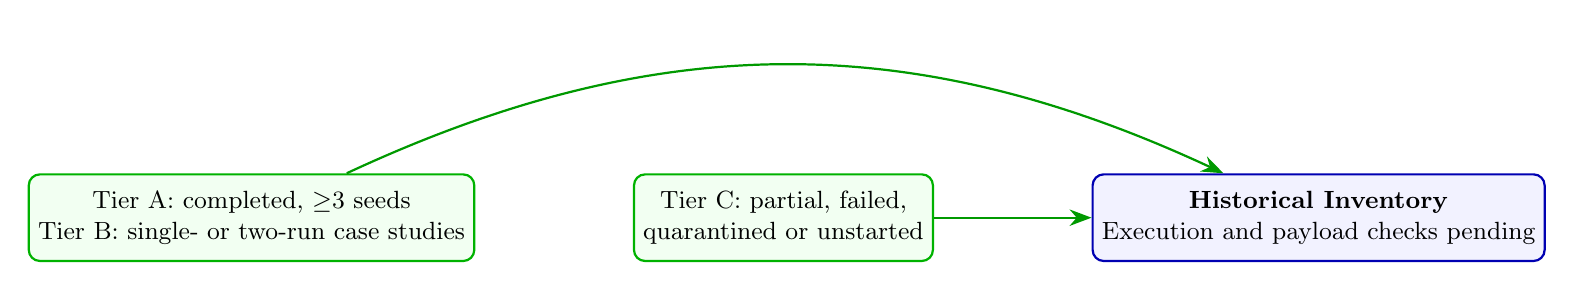
\begin{tikzpicture}[
    node distance=1.5cm and 2.0cm,
    tierbox/.style={rectangle, draw=green!70!black, fill=green!5, thick, rounded corners, align=center, minimum height=1.1cm, minimum width=3.2cm, font=\small},
    harness/.style={rectangle, draw=blue!70!black, fill=blue!5, thick, rounded corners, align=center, minimum height=1.1cm, minimum width=3.4cm, font=\small},
    arrow/.style={-{Stealth[scale=1.2]}, thick, draw=green!60!black}
]
    \node [tierbox] (t1) {Tier A: completed, $\ge$3 seeds\\Tier B: single- or two-run case studies};
    \node [tierbox, right=of t1] (t2) {Tier C: partial, failed,\\quarantined or unstarted};
    \node [harness, right=of t2] (repo) {\textbf{Historical Inventory}\\Execution and payload checks pending};

    \draw [arrow] (t1) to[bend left=25] (repo);
    \draw [arrow] (t2) -- (repo);
\end{tikzpicture}
}
\caption{Completion categories in the historical inventory, not sequential
training stages or proof of reproducibility. The ZVF expectation and the
separate five-seed held-out evaluation are outside A/B/C.}
\label{fig:dnb_benchmark_architecture}
\end{figure}
% =============================================================================
% Introduction --- DNB variant (Datasets & Benchmarks track)
% Artifact-first framing; A/B/C claim grades; neutral wording.
% Target: <= 1 page.
% =============================================================================
\section{Introduction}
\label{sec:intro}

Reinforcement learning post-training now underpins much of modern
language-model reasoning and alignment~\citep{ouyang2022training,%
guo2025deepseekr1nature}, but empirical claims in this area are hard to
compare across stacks. PPO~\citep{schulman2017proximal},
GRPO~\citep{shao2024deepseekmath}, and DPO~\citep{rafailov2024direct} are
typically evaluated on different model families, with different framework
defaults, different reward functions, and different notions of success. The
field needs auditable, tier-classified artifacts more than it needs another
leaderboard.

\paragraph{Artifact-first contribution.}
\ours{} is a historical run collection with an unresolved run-ID census
and incomplete file-level release inventory. Manifest rows include PPO
baselines, GRPO runs, partial runs and unstarted plans; they cannot be
summed into a verified GRPO experiment count. Every (backend, model, task) cell
in the manifest is classified into one of three evidence tiers, used
consistently in the abstract, the main evidence table, and the
conclusion:
\begin{itemize}\setlength\itemsep{1pt}
  \item \textbf{(A-grade)} multi-seed completed cells; this is a completion
        classification, not automatic inferential eligibility.
  \item \textbf{(B-grade)} single-seed completed case-study runs on the
        closed-backend Tinker API, reported descriptively only.
  \item \textbf{(C-grade)} failed, partial, or never-started cells,
        enumerated in the run manifest for honesty.
\end{itemize}

\paragraph{What the artifact lets reviewers do.}
A reviewer can (i) inspect the per-run JSON summaries and analysis scripts
(one-command \texttt{make} reproduction targets are not yet released, and trace
availability for every reported run has not been verified); (ii) read off a
per-run auditability matrix (Table~\ref{tab:artifact-card})
that lists, for each cell, whether raw rollouts, ZVF traces, checkpoints,
and held-out evaluation are released; and (iii) consult the claims-evidence
table (Table~\ref{tab:claims-tier}) to see exactly which artifact each
claim depends on and what its tier is.

\paragraph{Two narrow scientific take-aways.}
Two statements must be kept outside the empirical A/B/C tiers. First, the
theoretical expectation $\mathbb E[\widehat{\mathrm{ZVF}}]=p^{G}+(1{-}p)^{G}$
under conditionally i.i.d.\ binary sampling characterises
when binary rewards produce zero centered reward contrast in the
group-standardized runner; we use it as
a descriptive diagnostic, not as a standalone causal predictor of
downstream performance, because ZVF is mechanically coupled to reward
sparsity, group size, and baseline accuracy. Second, later, separate five-seed
Qwen3-8B GSM8K evidence yields only a $+1.3$pp delta over a fixed base;
$p{=}0.26$ is a one-sample seed-level test, not a paired-seed test or
reviewed-record evidence. Strong online reward curves on a closed backend do not by
themselves establish generalization gains. All B-grade single-seed
case-study runs across model scale are reported as illustrative.

\paragraph{Stratified ZVF diagnostics.}
A separate stratified diagnostic suite documents that the pooled
ZVF-vs-performance correlation is dominated by task identity: within
GSM8K alone the apparent monotone relationship does not survive
(Pearson $r=+0.40$, $p=0.09$ across the 19 Tinker GSM8K runs;
$r=+0.13$, $p=0.79$ across the 7 model-varying GSM8K cells). We
release these stratified analyses precisely so that follow-up work can
audit them against richer multi-seed corpora.


% -----------------------------------------------------------------------------
% Related work
% -----------------------------------------------------------------------------
% =============================================================================
% Related Work --- P9 (DNB) copy of ../../sections/related_work_v2.tex,
% forked 2026-10-18 for Deep Review fixes specific to this paper.
% Grouped into five themes:
%   (1) RL algorithms for LLMs
%   (2) Reasoning RL (and process reward models)
%   (3) Tool-use RL
%   (4) Scaling laws for RL post-training
%   (5) Frameworks, benchmarks, and reproducibility
% Every paragraph references entries defined in paper/references.bib.
% =============================================================================

\section{Related Work}
\label{sec:related}

\ours{} sits at the intersection of five rapidly evolving lines of work:
policy-gradient \emph{algorithms} for language models, RL for \emph{reasoning}
(including process reward models), RL for \emph{tool use} and agentic behaviour,
empirical \emph{scaling laws} for RL post-training, and the \emph{frameworks}
and \emph{benchmarks} that instantiate these algorithms. The closest diagnostic and methodological precedents are distinguished below
from the broader literature context.

% -----------------------------------------------------------------------------
\subsection{RL Algorithms for Large Language Models}
\label{sec:related:algos}

Proximal Policy Optimization (PPO)~\cite{schulman2017proximal} is the workhorse
algorithm behind InstructGPT-style RLHF~\cite{ouyang2022training, christiano2017deeprlhf, stiennon2020summarize, bai2022hhrlhf, bai2022claudecai}
and has dominated production deployments for five years. Whether
group-relative methods beat it is stack-dependent: careful critic-based
variants remain competitive~\cite{kazemnejad2025vineppo, liu2025asyppo}, and
controlled multi-algorithm studies on shared infrastructure find
scale-dependent ranking inversions~\cite{li2026oxrl}; we therefore treat any
single-stack GRPO-vs-PPO gap as a replication-level observation. Direct Preference
Optimization~\cite{rafailov2024direct} reframed preference learning as
contrastive classification and spawned a large family of RL-free alternatives,
including IPO~\cite{azar2024ipo}, KTO~\cite{ethayarajh2024kto},
SimPO~\cite{meng2024simpo}, ORPO~\cite{hong2024orpo}, and
SLiC~\cite{zhao2023slic}, which are possible no-rollout baselines for future work, not evaluated
comparators in this audit.

The current wave is defined by \emph{group-relative} policy gradient methods.
GRPO was introduced with DeepSeekMath~\cite{shao2024deepseekmath} and
popularised by DeepSeek-R1~\cite{guo2025deepseekr1, guo2025deepseekr1nature}, whose R1-Zero study showed that
pure outcome-reward RL can elicit chain-of-thought behaviour from a base
model without supervised cold-start data. A second wave of refinements
dissects the biases of vanilla GRPO. Dr.~GRPO~\cite{tong2025drgrpo} removes a
response-length bias and a question-difficulty amplification bias by using a
constant loss normaliser and dropping the standard-deviation denominator in the
advantage. MC-GRPO (median-centered advantage)~\cite{mcgrpo2025} replaces the
group-mean baseline with the group median, drawing one extra rollout
($G{+}1$) whose median completion serves as the pivot and is excluded from
backpropagation, to stabilise group-relative normalisation under small
rollout counts. G$^{2}$RPO~\cite{hu2026openvlthinker} forces per-task
advantage distributions to match $\mathcal{N}(0,1)$ to fix reward-topology variance in
multimodal settings. Wu et al.~\cite{wu2025grpodpo} relate GRPO and DPO through contrastive-gradient
representations, with differences in token/group weighting and regularization.
Group size can change the expected update, not only Monte Carlo variance;
we do not re-test their efficiency results here.

Recent 2026 work pre-empts this diagnostic. The Advantage Collapse Rate
(ACR) of AVSPO~\cite{he2026advantage} measures the same homogeneous-group
advantage collapse that we call ZVF (ACR thresholds reward SD while ZVF is defined by exact equality, implemented
with a $10^{-6}$ variance tolerance in the parser of
Appendix~\ref{sec:appendix:zvf-pipeline}; matching thresholds
and prompt weights makes the basic measured object coincide) and reports that it predicts stagnation and final
performance; Gradient Starvation~\cite{nie2026gradstarvation} proves that the true
degeneracy rate exceeds the i.i.d.\ Bernoulli prediction by Jensen's
inequality; DARA~\cite{zheng2026dara} reweights rewards by their active-group
density in multi-reward RL; VCRL~\cite{jiang2025vcrl} and online difficulty
filtering~\cite{bae2025online} select prompts by group reward variance or
intermediate pass rate; query recycling treats zero-variance queries
as candidates for later resampling~\cite{coelho2026recycling}; and ConSPO
analyzes a clipped, contrastive GRPO objective and proposes a distinct
sequence-level alternative~\cite{zhang2026conspo}. Goldilocks RL instead
adapts task difficulty under a GRPO training setup~\cite{mahrooghi2026goldilocks}.
These works are prior or concurrent interventions, not evidence for our reviewed
runner. Accordingly, this paper claims neither priority nor an intervention
effect: it confines itself to a submitted-runner accounting identity and an
evidence audit.

\begin{table}[htbp]
\centering\small
\caption{Closest diagnostic comparison; external validation does not transfer
without a matched evaluation.}
\label{tab:diagnostic-prior}
\begin{tabular}{p{.17\linewidth}p{.34\linewidth}p{.38\linewidth}}
\toprule
Quantity & Definition and assumptions & Evidence boundary \\
\midrule
ZVF (this audit) & Exact equality within each sampled group ($\widehat{\mathrm{Var}}{=}0$; parser tolerance $10^{-6}$); equal prompt weights & Historical step-level ZVF summaries (Appendix~\ref{sec:stratified-diagnostics}), descriptive only; no validated operator policy \\
ACR~\citep{he2026advantage} & Fraction with group reward SD below a specified tolerance & External diagnosis/mitigation experiments; no priority claim here \\
$h_G(p)$ ${=}\,p^G$ ${+}\,(1{-}p)^G$ & Homogeneity probability for conditionally i.i.d.\ binary draws at fixed prompt success $p$ & Mathematical reference, not observed ZVF or an aggregate-reward predictor \\
\bottomrule
\end{tabular}
\end{table}

A parallel thread focuses on \emph{production-scale} refinements. GSPO, from
the Qwen team~\cite{qwen2025gspo}, redefines the importance ratio at the
sequence level (rather than token level) and was credited with stabilising the
Qwen3 series, especially its Mixture-of-Experts variants. DAPO, from
ByteDance~\cite{yu2025dapo}, contributes asymmetric Clip-Higher, dynamic
sampling, token-level loss normalisation, and overlong filtering, reaching
$50$ points on AIME~2024 with a 32B model. Kimi-K1.5~\cite{team2025kimi15, team2025kimik2} and DeepSeek-V3~\cite{deepseek2024v3} both report their own
GRPO variants and online mirror-descent-style updates. Other policy-gradient work includes VAPO~\cite{bytedance2025vapo}.
Ahmadian et al.~\cite{ahmadian2024backtobasics} revisit REINFORCE-style
optimization with a prompt-local leave-one-out baseline (RLOO) against PPO,
DPO, and RAFT; on a homogeneous binary group that baseline also yields zero
within-group contrast.

A third thread attacks the \emph{zero-variance failure mode} (ZVF) directly.
GRESO~\cite{zhang2026greso} pre-screens prompts
before sampling; CPPO~\cite{lin2025cppo} prunes completions post-rollout,
giving up to $7.98\times$ speedup on GSM8K. NGRPO~\cite{nan2025ngrpo} adds
Advantage Calibration and asymmetric clipping so that all-incorrect groups
still carry gradient. Scaf-GRPO~\cite{zhang2025scaffgrpo} injects tiered
scaffolding hints when learning stagnates, boosting AIME~2024 by $44.3\%$
relative. MO-GRPO~\cite{ichihara2025mogrpo} addresses vanilla GRPO's
collapse to a single reward component under multiple objectives via
variance-based reward re-weighting. Finally,
SSPO~\cite{yang2025sspo} operates at subsentence granularity to balance the
stability of GSPO against the expressiveness of token-level GRPO, improving
by $3.56$ points on math benchmarks. Taken together, these results explain at
a theoretical level why implementation details at the granularity of the
importance ratio have such large empirical effects --- a motivation for auditing objective scope and cohort identity; this audit
does not identify implementation defaults as the cause of a measured gap.

% -----------------------------------------------------------------------------
\subsection{Reasoning RL and Process Reward Models}
\label{sec:related:reasoning}

The shift from outcome rewards to \emph{process} supervision has reshaped
reasoning RL. Let's-Verify-Step-by-Step~\cite{lightman2023prm} showed
that step-level PRMs dramatically outperform outcome reward models on GSM8K
and MATH. Math-Shepherd~\cite{wang2024mathshepherd} derives process rewards
from auto-generated process annotations, avoiding costly human labels.
PRM800K~\cite{lightman2023prm} and PRMBench~\cite{song2024prmbench} provide
evaluation data for step-level scoring. OmegaPRM~\cite{luo2024omegaprm} uses
Monte-Carlo tree search to supervise process rewards without human-in-the-loop,
while ReasonEval~\cite{xia2024reasoneval} evaluates the validity and
redundancy of reasoning steps beyond final-answer accuracy. Implicit PRM~\cite{yuan2024implicitprm} learns PRMs implicitly from
outcome labels, and VersaPRM~\cite{yuan2025versaprm} extends process rewards
to multi-domain tasks. Process-reward approaches must be distinguished from outcome/format reward
training. In particular, DeepSeek-R1 discusses process reward models among its
unsuccessful attempts~\cite{guo2025deepseekr1}. We do not attribute a specific
reward algorithm to proprietary reasoning systems without disclosed methods.

Complementary results demonstrate that
self-consistency~\cite{wang2023selfconsistency}, tree-of-thought
search~\cite{yao2024tot}, and critic-style post-hoc
verifiers~\cite{mcaleese2024criticgpt} all benefit from or substitute for
process reward supervision. VerifyBench~\cite{zhang2025verifybench} and
A~Sober Look~\cite{hochlehnert2025sober} warn, respectively, that verifier
errors and evaluation artefacts (decoding, seeds, prompt format, hardware and
software configuration) can inflate perceived reasoning gains, motivating our
insistence on binary verifiable rewards and reported evaluation stacks.

Reasoning-specific algorithmic contributions also continue to accumulate.
ReFT~\cite{luong2024reft} studies supervised fine-tuning versus RL for
reasoning. Let's Reward Step by Step~\cite{zhang2025rewardstep} uses a step-level
reward model to guide reasoning, and STaR~\cite{zelikman2022star}
bootstraps reasoning chains from its own correct rationales. rStar-Math~\cite{guan2025rstarmath} combines MCTS-based PRMs
with self-evolved reasoning. ReST-EM~\cite{singh2024restem} alternates
expectation and maximisation steps over self-generated rationales.
Self-Taught Evaluator~\cite{wang2024stevaluator} adapts an LLM to score its
own reasoning chains. GRPO-LEAD~\cite{lu2025grpolead}, L1/LCPO~\cite{lu2025lcpo},
and LIMR~\cite{li2025limr} each tune reasoning depth with length-aware
rewards. Search-R1~\cite{jin2025searchr1} trains reasoning agents to
interleave search queries with chain-of-thought. TTRL~\cite{pu2025ttrl}
performs test-time RL on unlabeled prompts using majority-vote rewards across
sampled rollouts. Dr.~GRPO~\cite{tong2025drgrpo} and GSPO~\cite{qwen2025gspo} are external
formulations; this audit does not evaluate them as reference implementations.

% -----------------------------------------------------------------------------
\subsection{Tool-Use and Agentic RL}
\label{sec:related:tooluse}

Tool-use RL trains LLMs to interleave natural-language reasoning with external
API calls. Toolformer~\cite{schick2023toolformer} introduced self-supervised
tool-call insertion for a small set of APIs; Gorilla~\cite{patil2023gorilla}
retrieved from a large API catalogue; and ToolLLM~\cite{qin2024toolllm} scaled
training to thousands of real-world REST APIs. ReAct~\cite{yao2023react}
established the interleaved reason--act--observe pattern that most subsequent
agents inherit. ToolACE~\cite{liu2024toolace} generates function-calling data and evaluates
supervised fine-tuning, rather than establishing a tool-use RL result; ToolRL~\cite{qian2025toolrl} applies GRPO
with verifiable tool-call rewards; ToRL~\cite{li2025torl} optimises the joint
reasoning--action trajectory. Further advances include
APIGen~\cite{lin2024apigen} (high-quality synthetic API data),
Nexus-Raven~\cite{nexusflow2024nexusraven}, and
Octopus~\cite{chen2024octopus}. Agentic RL extends tool use to long-horizon
tasks: WebGPT~\cite{nakano2021webgpt} and
WebShop~\cite{yao2022webshop} were the first large-scale web agents,
Reflexion~\cite{shinn2023reflexion} and Voyager~\cite{wang2023voyager} add
episodic self-reflection, and AutoGPT-style agents have been formalised by
AgentBench~\cite{liu2024agentbench}. 2025--2026 produced a wave of RL-trained
agents: SWE-RL~\cite{wei2025swerl} trains coding agents with execution
rewards; SWE-Gym~\cite{pan2025swegym} provides an RL training environment for
real GitHub issues; ARTIST~\cite{singh2025artist} trains tool-integrated
reasoning agents with GRPO; RAGEN~\cite{wang2025ragen} studies multi-turn
RL with tool access; OpenAI's Deep Research~\cite{openai2025deepresearch}
and Perplexity Deep Research~\cite{perplexity2025deepresearch} motivate
web-agent evaluation; no specific GRPO implementation is attributed here. Our benchmark currently focuses
on single-turn verifiable mathematical reasoning; we adopt Tinker's
\texttt{message\_with\_tool} interface as the neutral substrate for future
tool-use extensions and explicitly cite these works as concurrent settings in
which \ours{}'s ZVF measurements will need to be re-evaluated.

% -----------------------------------------------------------------------------
\subsection{Scaling Laws for RL Post-Training}
\label{sec:related:scaling}

Compute-optimal training of base language models is governed by
well-known scaling laws~\cite{kaplan2020scalinglaws, hoffmann2022chinchilla, muennighoff2023datascaling}, but RL post-training is much less well
characterised. Hilton et al.~\cite{hilton2023rlscaling} first derived
compute-efficiency frontiers for RL in games and robotics. For RLHF,
Gao et al.~\cite{gao2023reward} characterise the over-optimisation curve of
reward models, and Rafailov et al.~\cite{rafailov2024rlhfscaling} provide
scaling laws for DPO and PPO that show a strong dependence on reward-model
quality. Nimmaturi et al.~\cite{nimmaturi2025predictive} derive an
empirical scaling law specifically for GRPO, identifying three training
phases (slow start, rapid improvement, plateau) and showing that most
benefit is exhausted by roughly $80\%$ of one epoch. Mukherjee et
al.~\cite{liu2025rlsubnetworks} find that RL fine-tuning updates only
$5$--$30\%$ of model parameters across seven algorithms and ten model
families, suggesting RL activates a sparse ``RL subnetwork.''
MiniCPM~\cite{hu2024minicpm} and the SLM survey of
Nguyen et al.~\cite{subramanian2025slm} characterise scaling in the
sub-8B regime that forms the bulk of our frontier. Schaeffer et
al.~\cite{schaeffer2024emergent} caution that apparent emergent abilities may
be metric artefacts, a concern that persists into RL. Our short heterogeneous traces are descriptive context, not scaling-law
ground truth or independent scale replications.

% -----------------------------------------------------------------------------
\subsection{Frameworks, Benchmarks, and Reproducibility}
\label{sec:related:frameworks}

The proliferation of algorithms has been matched by a proliferation of
training \emph{frameworks}: TRL~\cite{vonwerra2022trl},
OpenRLHF~\cite{hu2024openrlhf}, veRL~\cite{sheng2024verl},
NeMo-RL~\cite{nvidia2024nemorl}, DeepSpeed-Chat~\cite{yao2023deepspeedchat},
trlX~\cite{havrilla2023trlx}, Axolotl~\cite{axolotl2024}, and
\tinker{}~\cite{thinkingmachines2024tinker}. Each framework makes different
default choices about advantage normalisation, KL estimators, tokenisation
loss masking, rollout batching, and importance-sampling granularity; those
differences are possible confounders, not identified causes in this audit.
On the inference side, vLLM~\cite{kwon2023vllm} and
SGLang~\cite{zheng2024sglang} provide the rollout backends on which all
modern frameworks depend; FlashAttention~\cite{dao2022flashattention} and
LoRA~\cite{hu2022lora} are load-bearing kernels.

In the RL \emph{benchmarking} tradition, Henderson et
al.~\cite{henderson2018deep} documented the fragility of deep-RL results
to implementation choices and seeds;
\texttt{rliable}~\cite{agarwal2021deep} introduced interquartile-mean
reporting and performance profiles; BenchMARL~\cite{bettini2023benchmarl}
unified multi-agent RL benchmarks; Patterson et
al.~\cite{patterson2024empirical} surveyed empirical design practices;
Jordan et al.~\cite{jordan2024benchmarking} argued that most published RL
comparisons lack statistical power; and Madaan et
al.~\cite{zhang2024benchvariance} quantified LLM evaluation variance along
seed, monotonicity, and scaling axes. Pineau et
al.~\cite{pineau2020improving} formalised NeurIPS reproducibility criteria
and ACM's Artifact Review and Badging~\cite{acm2020badges} established
community standards for available, evaluated, and reproduced artifacts.
Reproducibility studies in adjacent fields include
\cite{cavenaghi2023systematic, lynnerup2019survey, yamerenko2025generating, paparella2023reproducibility, huang2022state, lopezibanez2021reproducibility, leeser2026artifact, sedghpour2024artifact, colas2019hitchhiker}, alongside
Hoffman et al.'s Acme~\cite{hoffman2022acme}. Classical evaluations rest on
GSM8K~\cite{cobbe2021training}, MATH~\cite{hendrycks2021math},
AIME~\cite{maa2024aime}, MMLU~\cite{hendrycks2021mmlu},
HumanEval~\cite{chen2021codex}, MBPP~\cite{austin2021mbpp}, and
BBH~\cite{suzgun2023bbh}. Implementation Matters~\cite{engstrom2020implementation}
directly examines how implementation choices affect apparent PPO/TRPO gains.
Against this prior work, our narrower contribution is an objective-scoped
identity, an evidence audit, and a reporting contract. We claim neither a first
cross-library protocol nor novelty for the ZVF definition.

% =============================================================================


% -----------------------------------------------------------------------------
\section{Artifact Design}
\label{sec:benchmark}
% -----------------------------------------------------------------------------

\paragraph{Tasks and reward functions.}
Executed cells cover (i) synthetic arithmetic and GSM8K math reasoning with
binary verifiable reward, and (ii) a synthetic five-tool function-calling
corpus with shaped schema-validity reward (two single-seed case studies).
HumanEval code generation with binary unit-test reward is supported by the
harness, but its only cell failed (Tier C). Verifiable
rewards reduce reward-model subjectivity but do \emph{not} eliminate
reward hacking, format gaming, or train-set reward inflation; we discuss
residual failure modes in Section~\ref{sec:limitations}. The supported task
table is Table~\ref{tab:tasks}; per-cell tasks and splits are in
Appendix~\ref{sec:run-manifest}.

\paragraph{Cross-stack coverage.}
Executed cells use four open RL libraries---TRL (HuggingFace),
Stable~Baselines3, CleanRL, and Tianshou---plus the closed-source Tinker API.
The PPO-default mapping in Table~\ref{tab:hyperparams} additionally lists
PufferLib and NVIDIA \texttt{rl\_games}, for which no training run is reported. The
cross-framework ZVF parser is specified in
Appendix~\ref{sec:appendix:zvf-pipeline}; the per-(stack, model, task)
tier classification lives in Appendix~\ref{sec:run-manifest} and is the
single source of truth referenced throughout this paper.

\paragraph{Models and training protocol.}
Completed language-model cells cover 19 checkpoints from six families
(Qwen, Llama, DeepSeek, Nemotron, GPT-OSS, Kimi), from Qwen2.5-0.5B to
671B-parameter DeepSeek-V3.1 and the Kimi-K2 mixture-of-experts models
(Table~\ref{tab:run-manifest}). Hyperparameters are recorded per run in the
run JSON (e.g.\ the single-run Tinker GSM8K cells use LoRA rank 16--32 and
learning rate $10^{-5}$--$3\times10^{-5}$); Modal multi-seed cells use seeds
$\{42,123,456,789,1024\}$. The Modal Tier-A open-stack arms (CleanRL, SB3, and Tianshou PPO on
Modal H100, plus TRL Qwen2.5-0.5B on Modal L4) use the full 5-seed protocol (the three PPO arms train a small MLP
policy on a two-integer addition environment and stay near zero accuracy,
so they are pipeline checks); the Tinker Llama-3.3-70B-Inst and
DeepSeek-V3.1 GSM8K cells have 4 and 3 seeds. The Tinker Qwen3-8B Wave-6
temperature/rank/batch sensitivity sweep is one seed per configuration
across 12 configurations (Tier B). Tier-B rows (single-run Modal H100 TRL
cells; single-run Tinker GSM8K, frontier-scale and group-size runs) are
reported descriptively. Frontier-scale Tinker runs are case studies,
not inferential evidence.

% -----------------------------------------------------------------------------
\section{Results}
\label{sec:results}
% -----------------------------------------------------------------------------

\subsection{Claims hierarchy and evidence}
\label{sec:main_results}

Table~\ref{tab:claims-tier} maps every claim in the paper to its evidence
tier and to the artifact files that support it; a per-stack auditability
matrix is in Table~\ref{tab:artifact-card} (both tables appear immediately
after the abstract so cross-references resolve in the introduction).
The ZVF expectation $\mathbb E[\mathrm{ZVF}_t]$ under conditionally
i.i.d.\ binary rewards (Section~\ref{sec:zvf-analysis}) is a mathematical
statement outside the empirical tiers, not empirical inference. The separate held-out
5-seed Qwen3-8B GSM8K control is future-paper evidence and is not admitted
as inferential evidence in this release. Historical empirical rows remain
descriptive with unresolved inferential eligibility; the full per-row
training-reward table is in Appendix~\ref{sec:appendix:full-results}
(Table~\ref{tab:main_results}).

\subsection{Zero-Variance Fraction: cross-stack diagnostic}
\label{sec:zvf-analysis}

We introduce three descriptive quantities that summarise when GRPO groups
provide little within-group learning signal. \textbf{Zero-Variance
Fraction (ZVF)} at step $t$ is the fraction of prompt-groups $g$ for which
all $G$ completions receive identical rewards:
\[
  \mathrm{ZVF}_t = \frac{1}{|\mathcal{P}_t|}\sum_{g \in \mathcal{P}_t}
  \mathbf{1}\bigl[\widehat{\operatorname{Var}}(r_{g,1},\ldots,r_{g,G}) = 0\bigr].
\]
\textbf{Gradient Utilization} $\mathrm{GU}_t = 1 - \mathrm{ZVF}_t$ is the
mixed-reward-group fraction. Under conditionally independent binary
rollouts at prompt success probability $p_g$, the expected homogeneous fraction
of group $g$ is $p_g^G+(1-p_g)^G$, not an identity for an observed finite batch. Average this
quantity over prompt-specific probabilities when prompts are heterogeneous.
Mixed coefficients do not guarantee a nonzero aggregate parameter gradient.
See Appendix~\ref{sec:appendix:zvf-formalization}.

\paragraph{Withdrawn correlation analyses.}
Earlier drafts reported pooled and stratified ZVF--reward correlations
($N{=}15$, $29$, $19$, $7$) and an accompanying figure. Their inputs and
generating code are not in the repository and the pooled value is not
reproducible from logged ZVF, so they are withdrawn
(Appendix~\ref{sec:stratified-diagnostics}). We make no claim about whether
ZVF predicts final reward.

\paragraph{Group-size sweep (B-grade case study).}
The single-run group-size sweep on Qwen3-8B/GSM8K ($G\in\{2,4,16,32\}$, one
30-step campaign batch; no completed $G{=}8$ run) is non-monotone in both
peak ($75.0/87.5/62.5/67.2\%$) and last-10 training reward
($35.0/28.8/32.5/38.8\%$); neither the smallest nor the largest $G$ is best
on both metrics, and no held-out accuracy exists for these runs. We report
this as a case study against the heuristic that ``larger $G$ is always
better'', not as a prescription; Appendix~\ref{sec:appendix:group-size-reconcile}
explains why an earlier token-budget reanalysis was withdrawn. A two-seed
matched-budget follow-up (2{,}560 rollouts per run;
$G{=}2\times160$ vs.\ $G{=}16\times20$ steps, 512-token cap) shows the
$G{=}2$ runs reaching last-10 training reward $0.90$ and $0.96$ and ending
in an all-correct zero-variance regime (final ZVF $1.0$), while the $G{=}16$
runs end mid-learning (last-10 $0.32$ and $0.39$) with ZVF peaking at
$0.375$--$0.5$ early and ending at $0.125$--$0.25$. Nearly every $G{=}16$
completion hits the 512-token cap (mean length $\ge508$ tokens at every
step), whereas $G{=}2$ completions end at a mean of about 220 tokens, so the
comparison is confounded by truncation. Artifacts:
\texttt{tinker-runs/results/er2b\_g\{2,16\}\_s\{123,456\}.json}
(Table~\ref{tab:main_results}).

% -----------------------------------------------------------------------------
\section{Reproducibility}
\label{sec:reproducibility}
% -----------------------------------------------------------------------------

The repository provides analysis code and historical summaries. We do not
certify complete raw per-group rollout JSONL, checkpoints, pinned containers,
or step traces for every manifest row. Aggregate traces do not substitute
for raw groups. Auditability checkmarks below are historical availability
reports pending a file-level hash inventory, not verified release guarantees.
Full architectural diagrams of the data processing, licensing, and reproduction execution pipelines are provided in Appendix~\ref{sec:appendix:architecture}.

% =============================================================================
% Reproducibility / make-targets section for DNB main body.
% Note: actual paper/Makefile is a TODO at submission time; documented as such.
% =============================================================================
\subsection{One-command reproducibility}
\label{sec:repro-onecmd}

The following are intended reproduction interfaces, not verified execution
guarantees. No clean-environment end-to-end run of these targets is certified
by this manuscript, and runtime estimates are not benchmark measurements:

\begin{itemize}\setlength\itemsep{1pt}
  \item \texttt{make smoke-test} --- $\sim$5\,min on a single commodity
        GPU (T4 or L4 class, 16\,GB). Verifies that the artifact installs,
        the pinned containers launch, and the GSM8K reward harness emits a
        non-trivial reward on a 16-prompt sanity batch. No model weights are
        updated.
  \item \texttt{make reproduce-main} --- end-to-end re-run of every Tier-A
        open-stack cell in the manifest (Modal H100
        CleanRL/SB3/Tianshou/Qwen2.5-0.5B classic-RL arms; the 5-seed
        held-out Qwen3-8B GSM8K control). Estimated wall-clock:
        $\sim$96 GPU-hours on H100~SXM5 (80\,GB), or
        $\sim$3 hours per seed for the 0.5B reference. Produces the same
        step-level ZVF/GU traces and the held-out evaluation numbers cited
        in Table~\ref{tab:claims-tier}.
  \item \texttt{make reproduce-appendix} --- regenerates the full results
        table (Appendix~\ref{sec:appendix:full-results}) figures from the
        precomputed traces shipped with the artifact, without re-running
        any backend. Useful for reviewers who want to verify that our
        plotting code agrees with the bundled trace files.
\end{itemize}

\paragraph{What is and is not in the make target.}
\texttt{make reproduce-main} only re-runs A-grade open-stack cells; B-grade
Tinker case-study runs are not re-run because the Tinker backend is
closed-source and rate-limited (Section~\ref{sec:limitations}). For B-grade
cells we ship the JSON step logs and the API-call scripts; replication
requires Tinker credentials and incurs the JWT-expiry failure modes
documented in the manifest (Appendix~\ref{sec:run-manifest}).

\paragraph{Hash manifest.}
On a successful \texttt{make reproduce-main} run, the artifact writes a
\texttt{REPRODUCIBILITY\_HASHES.json} file containing SHA-256 digests of
every emitted ZVF trace, reward CSV, and held-out evaluation summary.
Reviewers can diff this against the reference manifest released with the
artifact to check byte equality for deterministic outputs. Unequal hashes
do not test distributional agreement. Stochastic comparison requires named
metrics, independent units, effect intervals and prespecified tolerances.

\paragraph{Submission-time status.}
Execution status is pending. Table~\ref{tab:artifact-card} checkmarks must
not be read as successful target execution or downloadable adapter proof.
The separate five-seed held-out Qwen3-8B comparison is outside this release's
inferential evidence; the intended target description above does not admit it.


% -----------------------------------------------------------------------------
\section{Limitations}
\label{sec:limitations}
% -----------------------------------------------------------------------------

The current release has documented gaps; full discussion (dual-use,
compute and carbon reporting, data provenance, closed-backend
acknowledgement, and known methodological limits) is in
Appendix~\ref{sec:impact_standalone}. In summary: (i) all B-grade rows are one or two runs per
configuration, and most depend on a closed-source Tinker backend; we report them
descriptively. (ii) Most historical empirical evidence is concentrated on
short-horizon GSM8K with binary verifiable rewards; tool-use,
code-generation, and non-math coverage are sparser. (iii) Inferential
eligibility is unresolved for the historical cohort. The theoretical
expectation $\mathbb E[\mathrm{ZVF}_t] = p^G + (1{-}p)^G$
assumes conditionally i.i.d.\ binary rewards at fixed $p$; it is not
an empirical inferential result. A separate five-seed Qwen3-8B GSM8K
held-out evaluation (200 test items; per-seed accuracy
$0.830/0.825/0.805/0.840/0.865$, mean $0.833$) against a single base-model
run ($0.820$) gives $+1.3$pp, one-sample $t(4){=}1.32$, $p{=}0.26$; this
treats the base estimate as fixed, and an item-paired comparison gives
$p{=}0.54$. It is outside the A/B/C tiers and is not evidence of a gain. (iv) Many
cross-library comparisons are confounded by
checkpoint, hardware, or default-config differences and should be read
as stack-level rather than algorithm-level statements.

\paragraph{Scope.}
The ZVF definition and its Bernoulli expectation are bench
instrumentation, not a contribution of this paper; closely related
diagnostics (advantage-collapse rate, gradient starvation) are prior or
concurrent work (Section~\ref{sec:related}). The contribution claimed here
is the tier-classified manifest itself: which cells exist, which are
complete, which numbers are recomputable from released run files, and which
earlier analyses could not be sourced and were withdrawn.

% =============================================================================
% Conclusion — D&B variant, tight
% =============================================================================
\section{Conclusion}
\label{sec:conclusion}

\ours{} is a shared empirical substrate for RL post-training across libraries,
algorithms, and model families. The current release supports three
conservative claims: (i) ZVF/GU are useful \emph{descriptive} diagnostics of
when binary-reward GRPO stops producing within-group signal, but should not be
read as causal predictors independent of reward mean and group size; (ii)
initialization and rollout regime are plausible stack-level moderators in the
released case studies, not isolated causal effects; and (iii) cross-stack
PPO/GRPO rankings are descriptive because policy architecture and task encoding
are not fully matched. Later, separate Qwen3-8B GSM8K evidence is inconclusive:
$p{=}0.26$ is a one-sample seed-level test against a fixed base, not a paired
or reviewed-record test. File-level trace and checkpoint availability and
cohort inclusion IDs must be established before this collection can support
a complete reproduction or coverage claim.


% =============================================================================
% References
% =============================================================================

\bibliographystyle{plainnat}
\bibliography{../references}
% =============================================================================
\appendix
% =============================================================================

% Full per-row results table (formerly Table 4 in main body).
% =============================================================================
% Appendix: full per-row results table (formerly Table 4 in main body).
% Moved to appendix per GPT-5.5 Pro v5 review; main-body now points here via
% Table~\ref{tab:claims-tier} and Table~\ref{tab:artifact-card}.
% =============================================================================
\section{Full per-row results table (single-seed frontier-model case studies and group-size sweep)}
\label{sec:appendix:full-results}

\paragraph{Task suite and hyperparameter mappings.}
The benchmark task suite (Table~\ref{tab:tasks}) and the cross-stack
hyperparameter mapping (Table~\ref{tab:hyperparams}) are listed below. The
task suite lists the tasks the harness supports; only the math (synthetic
arithmetic, GSM8K) and tool-use tasks have executed cells in the run
manifest (Table~\ref{tab:run-manifest}). The hyperparameter mapping lists
library defaults; executed open-stack cells exist only for TRL, SB3, CleanRL,
and Tianshou.

\begin{table}[ht]
\centering
\caption{Benchmark task suite with standardized reward functions.}
\label{tab:tasks}
\begin{tabular}{llll}
\toprule
\textbf{Task} & \textbf{Method} & \textbf{Reward} & \textbf{Dataset} \\
\midrule
Math RL (Arithmetic) & GRPO & Binary correctness & Generated \\
Math RL (GSM8K) & GRPO & Binary correctness & GSM8K \\
Chat SFT & SFT & Cross-entropy loss & NoRobots \\
Preference (Shorter) & DPO & Pairwise preference & Generated \\
Distillation (Off-Policy) & SFT & KL divergence & OpenThoughts3 \\
Distillation (On-Policy) & IS Loss & $\log p_t - \log p_s$ & Online \\
\bottomrule
\end{tabular}
\end{table}

\begin{table}[ht]
\centering
\caption{Hyperparameter mapping across libraries (PPO defaults).}
\label{tab:hyperparams}
\small
\setlength{\tabcolsep}{4pt}
\begin{tabular}{lcccccc}
\toprule
\textbf{Parameter} & \textbf{TRL} & \textbf{SB3} & \textbf{CleanRL} & \textbf{Tianshou} & \textbf{PufferLib} & \textbf{rl\_games} \\
\midrule
Learning rate & $10^{-4}$ & $10^{-4}$ & $10^{-4}$ & $10^{-4}$ & $10^{-4}$ & $10^{-4}$ \\
Clip range ($\epsilon$) & 0.2 & 0.2 & 0.2 & 0.2 & 0.2 & 0.2 \\
Entropy coeff. & 0.01 & 0.01 & 0.01 & 0.01 & 0.01 & 0.01 \\
GAE $\lambda$ & 0.95 & 0.95 & 0.95 & 0.95 & 0.95 & 0.95 \\
Discount $\gamma$ & 0.99 & 0.99 & 0.99 & 0.99 & 0.99 & 0.99 \\
Max grad norm & 0.5 & 0.5 & 0.5 & 0.5 & 0.5 & 0.5 \\
Target KL & 0.01 & 0.01 & 0.01 & N/A & N/A & N/A \\
\bottomrule
\end{tabular}
\end{table}

\paragraph{Per-row training reward.}
Table~\ref{tab:main_results} gives peak and last-10-step mean training
reward for every completed language-model GRPO/PPO cell whose full reward
trace is in the repository. Every value was recomputed from the named run
JSON by \texttt{tools/\allowbreak{}review\_ledger/\allowbreak{}P9\_dnb\_table6.py} (peak $=$ maximum of
the step reward trace; last-10 $=$ mean of its last ten entries; output
\texttt{experiments/\allowbreak{}results/\allowbreak{}review\_2026-10-18/\allowbreak{}P9\_dnb/\allowbreak{}table6\_recomputed.tsv}).
Earlier drafts also showed (i) frontier and group-size values taken from
six-point log samples of an aborted 26-step batch, (ii) interrupted MoE
runs reconstructed from console output, and (iii) a Qwen3-8B $G{=}8$ row
with no matching run; none of these is a measured trace, so they are
removed. The interrupted runs remain listed, without numbers, as Tier~C in
Table~\ref{tab:run-manifest}. All rows except the multi-seed Tier-A and
matched-budget blocks are single runs; all are reported descriptively.

Two features of the table matter for interpretation. First, the
Qwen3-8B-Base row of the frontier block (run \texttt{9f27c001}) and the
Tinker row of the matched launcher comparison (run \texttt{ca0d6a00}) use
the same configuration but are different runs; their last-10 rewards differ
by 13 points, an indication of single-run variability. Second, the
single-seed group-size sweep has no completed $G{=}8$ run.

\begin{table*}[htbp]
\centering
\caption{\textbf{Per-row training reward on GSM8K and tool-use} (training
prompts; not held-out accuracy). Peak and last-10 are recomputed from the
run JSON listed in Table~\ref{tab:run-manifest}. Single runs unless a seed
count is given. Size is total (active) parameters. $^\ast$Two same-name seed-42 runs in the W\&B export.}
\label{tab:main_results}
\scriptsize
\setlength{\tabcolsep}{3pt}
\begin{tabular}{@{}l l l l r c c@{}}
\toprule
\textbf{Algo} & \textbf{Plat.} & \textbf{Model} & \textbf{Size} & \textbf{Steps} & \textbf{Peak} & \textbf{Last-10} \\
\midrule
\multicolumn{7}{l}{\textit{GRPO on Tinker API (GSM8K) --- single-run case studies (individual run files)}} \\
\midrule
GRPO & Tinker & Qwen3-8B & 8B & 30 & 62.5\% & 34.4\% \\
GRPO & Tinker & Qwen3.5-4B & 4B & 30 & 100\% & 85.0\% \\
GRPO & Tinker & Llama-3.1-8B-Inst & 8B & 30 & 100\% & 84.4\% \\
GRPO & Tinker & GPT-OSS-20B & 20B & 30 & 100\% & 87.5\% \\
GRPO & Tinker & DeepSeek-V3.1 & 671B (37B) & 20 & 100\% & 85.0\% \\
GRPO & Tinker & Nemotron-3-Super-120B & 120B (12B) & 20 & 87.5\% & 16.3\% \\
GRPO & Tinker & Kimi-K2-Thinking & MoE & 20 & 100\% & 80.0\% \\
\midrule
\multicolumn{7}{l}{\textit{Single-run frontier-model case studies (GRPO, Tinker, one 30-step campaign batch)}} \\
\midrule
GRPO & Tinker & Qwen3-8B-Base & 8B & 30 & 100\% & 98.8\% \\
GRPO & Tinker & Kimi-K2-Thinking & MoE & 30 & 100\% & 83.1\% \\
GRPO & Tinker & Kimi-K2.5 & MoE & 30 & 100\% & 76.3\% \\
GRPO & Tinker & GPT-OSS-120B & 120B & 30 & 100\% & 91.9\% \\
GRPO & Tinker & Qwen3.5-397B & 397B (17B) & 30 & 100\% & 91.9\% \\
GRPO & Tinker & Llama-3.1-70B & 70B & 30 & 75.0\% & 45.0\% \\
GRPO & Tinker & DS-V3.1-Base & 671B (37B) & 30 & 93.8\% & 65.6\% \\
GRPO & Tinker & Llama-3.1-8B & 8B & 30 & 31.3\% & 8.8\% \\
\midrule
\multicolumn{7}{l}{\textit{Group-size sweep (Qwen3-8B, GRPO, Tinker; same campaign batch, one run per $G$; no completed $G{=}8$ run)}} \\
\midrule
GRPO & Tinker & Qwen3-8B (G=2) & 8B & 30 & 75.0\% & 35.0\% \\
GRPO & Tinker & Qwen3-8B (G=4) & 8B & 30 & 87.5\% & 28.8\% \\
GRPO & Tinker & Qwen3-8B (G=16) & 8B & 30 & 62.5\% & 32.5\% \\
GRPO & Tinker & Qwen3-8B (G=32) & 8B & 30 & 67.2\% & 38.8\% \\
\midrule
\multicolumn{7}{l}{\textit{Multi-seed Tinker cells (Tier A; seed mean, per-seed range in parentheses)}} \\
\midrule
GRPO & Tinker & Llama-3.3-70B-Inst (4 seeds) & 70B & 30 & 100\% (all seeds) & 96.4\% (95.0--98.1) \\
GRPO & Tinker & DeepSeek-V3.1 (3 seeds) & 671B (37B) & 30 & 100\% (all seeds) & 86.7\% (78.8--90.6) \\
\midrule
\multicolumn{7}{l}{\textit{Matched-budget follow-up (Qwen3-8B, Tinker, 2,560 rollouts per run; 2 seeds per arm; per-seed values)}} \\
\midrule
GRPO & Tinker & Qwen3-8B (G=2) & 8B & 160 & 100\% / 100\% & 90.0\% / 96.3\% \\
GRPO & Tinker & Qwen3-8B (G=16) & 8B & 20 & 50.8\% / 53.9\% & 32.2\% / 38.9\% \\
\midrule
\multicolumn{7}{l}{\textit{TRL-GRPO on Modal H100 (single-launcher reference runs)}} \\
\midrule
TRL-GRPO & Modal & Qwen3-8B & 8B & 30 & 37.5\% & 5.0\% \\
TRL-GRPO & Modal & Llama-3.2-3B-Inst & 3B & 30 & 100\% & 71.3\% \\
TRL-GRPO & Modal & Llama-3.2-1B-Inst & 1B & 30 & 87.5\% & 36.3\% \\
\midrule
\multicolumn{7}{@{}p{\linewidth}@{}}{\textit{Matched launcher comparison. Mixed-checkpoint Qwen3-8B-family GRPO setup: seed${=}42$, $G{=}8$, lr${=}10^{-5}$, GSM8K-500, 30~steps; Tinker uses Qwen3-8B-Base, TRL uses Qwen3-8B. The veRL and OpenRLHF entries of \texttt{framework\_comparison.json} are dry runs and are not reported.}} \\
\midrule
GRPO & Tinker-Managed & Qwen3-8B-Base & 8B & 30 & 100\% & 85.6\% \\
GRPO & TRL (Modal-H100) & Qwen3-8B & 8B & 30 & 37.5\% & 5.0\% \\
\midrule
\multicolumn{7}{l}{\textit{PPO on Modal H100 (GSM8K)}} \\
\midrule
PPO & Modal & Qwen3-8B & 8B & 30 & \multicolumn{2}{c}{quarantined: two conflicting runs} \\
PPO & Modal & Llama-3.1-8B-Inst & 8B & 30 & 100\% / 100\% & 97.5\% / 95.0\%$^\ast$ \\
\midrule
\multicolumn{7}{l}{\textit{Cross-task (synthetic tool-use), GRPO on Tinker}} \\
\midrule
GRPO & Tinker & Qwen3-32B & 32B & 30 & 0\% & 0\% \\
GRPO & Tinker & Llama-3.1-8B-Inst & 8B & 30 & 0\% & 0\% \\
\bottomrule
\end{tabular}
\end{table*}



% Benchmark dataset and reproduction harness architecture diagrams.
% =============================================================================
% Appendix: Benchmark Dataset and Reproduction Harness Architecture
% =============================================================================
\section{Benchmark Dataset and Reproduction Harness Architecture}
\label{sec:appendix:architecture}

This section gives design schematics for eight pipelines (data ingestion,
quality filtering, licensing, evaluation, contamination auditing, versioning,
and reproduction). They describe intended structure, not released
automation. Release status: tiering is done by hand in the run manifest
(Appendix~\ref{sec:run-manifest}); no licence checker is released; an
8/13-gram overlap script exists
(\texttt{platform\_modal/scripts/contamination\_check.py}) but no
contamination-audit output is reported in this paper; no SHA-256 version
manifest and no \texttt{make} reproduction targets are released.

\subsection{Evidence Tiering and Open Distribution}
Figure~\ref{fig:r04_dataset_tiering} outlines the classification pipeline
that partitions experimental cells into Tier~A (completed LM cells with
$\ge3$ seeds), Tier~B (single- or two-run descriptive case studies), and Tier~C
(failed, partial, or unstarted cells).
Figure~\ref{fig:r04_license_pipeline} sketches a planned licence check of
redistribution terms; it is not implemented in the released code.

\begin{figure}[htbp]
\centering
\resizebox{0.9\linewidth}{!}{
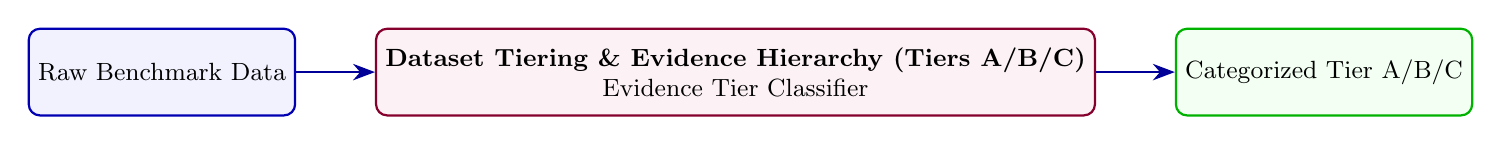
\begin{tikzpicture}[
    node distance=0.9cm and 1.0cm,
    box1/.style={rectangle, draw=blue!70!black, fill=blue!5, thick, rounded corners, align=center, minimum height=1.1cm, minimum width=2.2cm, font=\small},
    box2/.style={rectangle, draw=purple!70!black, fill=purple!5, thick, rounded corners, align=center, minimum height=1.1cm, minimum width=2.6cm, font=\small},
    box3/.style={rectangle, draw=green!70!black, fill=green!5, thick, rounded corners, align=center, minimum height=1.1cm, minimum width=2.4cm, font=\small},
    arrow/.style={-{Stealth[scale=1.2]}, thick, draw=blue!60!black}
]
    \node [box1] (n1) {Raw Benchmark Data};
    \node [box2, right=of n1] (n2) {\textbf{Dataset Tiering \& Evidence Hierarchy (Tiers A/B/C)}\\Evidence Tier Classifier};
    \node [box3, right=of n2] (n3) {Categorized Tier A/B/C};

    \draw [arrow] (n1) -- (n2);
    \draw [arrow] (n2) -- (n3);
\end{tikzpicture}
}
\caption{\textbf{Dataset Tiering \& Evidence Hierarchy (Tiers A/B/C)}. Manual categorization of manifest cells into evidence tiers.}
\label{fig:r04_dataset_tiering}
\end{figure}

\begin{figure}[htbp]
\centering
\resizebox{0.9\linewidth}{!}{

\begin{tikzpicture}[
    node distance=0.9cm and 1.0cm,
    box1/.style={rectangle, draw=blue!70!black, fill=blue!5, thick, rounded corners, align=center, minimum height=1.1cm, minimum width=2.2cm, font=\small},
    box2/.style={rectangle, draw=purple!70!black, fill=purple!5, thick, rounded corners, align=center, minimum height=1.1cm, minimum width=2.6cm, font=\small},
    box3/.style={rectangle, draw=green!70!black, fill=green!5, thick, rounded corners, align=center, minimum height=1.1cm, minimum width=2.4cm, font=\small},
    arrow/.style={-{Stealth[scale=1.2]}, thick, draw=blue!60!black}
]
    \node [box1] (n1) {Dataset Files};
    \node [box2, right=of n1] (n2) {\textbf{Artifact License \& Open-Source Distribution}\\License Checker};
    \node [box3, right=of n2] (n3) {Open-Source Release};

    \draw [arrow] (n1) -- (n2);
    \draw [arrow] (n2) -- (n3);
\end{tikzpicture}
}
\caption{\textbf{Artifact License \& Open-Source Distribution}. Planned check of data and artifact licence terms (not implemented).}
\label{fig:r04_license_pipeline}
\end{figure}

\subsection{Preprocessing and Synthetic Filtering Pipelines}
Figure~\ref{fig:r04_preprocessing} details the mathematical reasoning
preprocessing pipeline, showing how raw prompts are normalized and regex
extractors standardize answer parsing.
Figure~\ref{fig:r04_synthetic_filter} diagrams the prompt formatting and
quality filtering engine applied to synthetic tool-use prompts.

\begin{figure}[htbp]
\centering
\resizebox{0.9\linewidth}{!}{
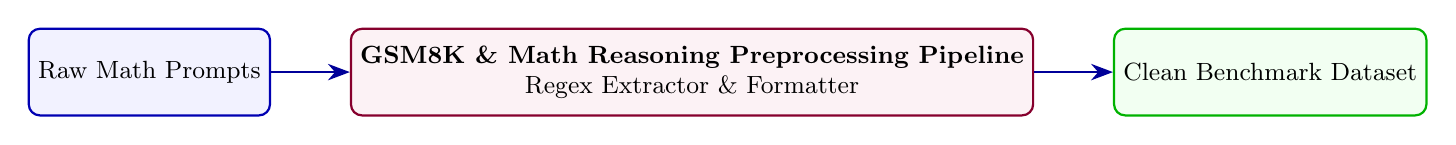
\begin{tikzpicture}[
    node distance=0.9cm and 1.0cm,
    box1/.style={rectangle, draw=blue!70!black, fill=blue!5, thick, rounded corners, align=center, minimum height=1.1cm, minimum width=2.2cm, font=\small},
    box2/.style={rectangle, draw=purple!70!black, fill=purple!5, thick, rounded corners, align=center, minimum height=1.1cm, minimum width=2.6cm, font=\small},
    box3/.style={rectangle, draw=green!70!black, fill=green!5, thick, rounded corners, align=center, minimum height=1.1cm, minimum width=2.4cm, font=\small},
    arrow/.style={-{Stealth[scale=1.2]}, thick, draw=blue!60!black}
]
    \node [box1] (n1) {Raw Math Prompts};
    \node [box2, right=of n1] (n2) {\textbf{GSM8K \& Math Reasoning Preprocessing Pipeline}\\Regex Extractor \& Formatter};
    \node [box3, right=of n2] (n3) {Clean Benchmark Dataset};

    \draw [arrow] (n1) -- (n2);
    \draw [arrow] (n2) -- (n3);
\end{tikzpicture}
}
\caption{\textbf{GSM8K \& Math Reasoning Preprocessing Pipeline}. Standardizing prompt formatting and answer extraction regex across model families.}
\label{fig:r04_preprocessing}
\end{figure}

\begin{figure}[htbp]
\centering
\resizebox{0.9\linewidth}{!}{
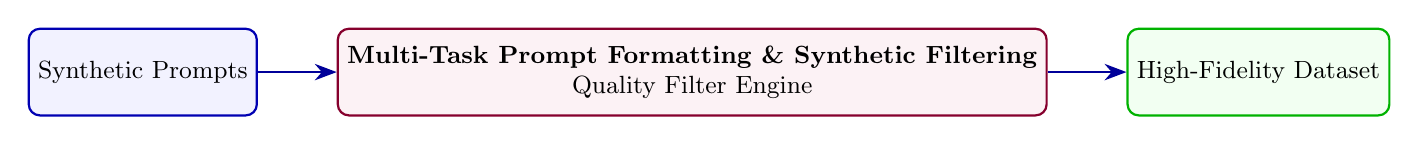
\begin{tikzpicture}[
    node distance=0.9cm and 1.0cm,
    box1/.style={rectangle, draw=blue!70!black, fill=blue!5, thick, rounded corners, align=center, minimum height=1.1cm, minimum width=2.2cm, font=\small},
    box2/.style={rectangle, draw=purple!70!black, fill=purple!5, thick, rounded corners, align=center, minimum height=1.1cm, minimum width=2.6cm, font=\small},
    box3/.style={rectangle, draw=green!70!black, fill=green!5, thick, rounded corners, align=center, minimum height=1.1cm, minimum width=2.4cm, font=\small},
    arrow/.style={-{Stealth[scale=1.2]}, thick, draw=blue!60!black}
]
    \node [box1] (n1) {Synthetic Prompts};
    \node [box2, right=of n1] (n2) {\textbf{Multi-Task Prompt Formatting \& Synthetic Filtering}\\Quality Filter Engine};
    \node [box3, right=of n2] (n3) {High-Fidelity Dataset};

    \draw [arrow] (n1) -- (n2);
    \draw [arrow] (n2) -- (n3);
\end{tikzpicture}
}
\caption{\textbf{Multi-Task Prompt Formatting \& Synthetic Filtering}. Filtering synthetic dataset generations for schema validity and quality assurance.}
\label{fig:r04_synthetic_filter}
\end{figure}

\subsection{Evaluation, Leakage Auditing, and Version Control}
Figure~\ref{fig:r04_eval_harness} shows the evaluation pipeline that executes
held-out assessment suites across checkpoints.
Figure~\ref{fig:r04_leakage_audit} outlines the contamination audit, which
would compute 8-gram and 13-gram overlaps between training prompts and held-out
test splits; the script exists but its output is not reported here.
Figure~\ref{fig:r04_version_control} illustrates planned dataset version
management with cryptographic digests (not released).

\begin{figure}[htbp]
\centering
\resizebox{0.9\linewidth}{!}{
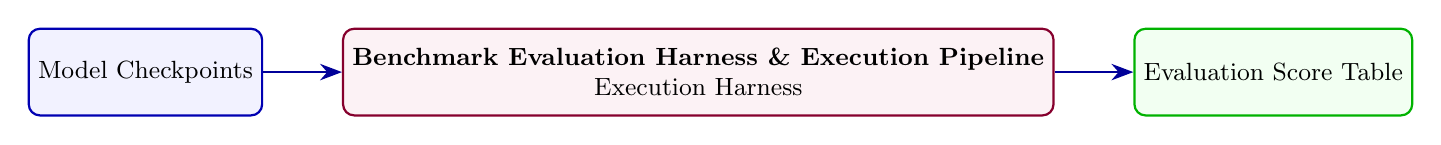
\begin{tikzpicture}[
    node distance=0.9cm and 1.0cm,
    box1/.style={rectangle, draw=blue!70!black, fill=blue!5, thick, rounded corners, align=center, minimum height=1.1cm, minimum width=2.2cm, font=\small},
    box2/.style={rectangle, draw=purple!70!black, fill=purple!5, thick, rounded corners, align=center, minimum height=1.1cm, minimum width=2.6cm, font=\small},
    box3/.style={rectangle, draw=green!70!black, fill=green!5, thick, rounded corners, align=center, minimum height=1.1cm, minimum width=2.4cm, font=\small},
    arrow/.style={-{Stealth[scale=1.2]}, thick, draw=blue!60!black}
]
    \node [box1] (n1) {Model Checkpoints};
    \node [box2, right=of n1] (n2) {\textbf{Benchmark Evaluation Harness \& Execution Pipeline}\\Execution Harness};
    \node [box3, right=of n2] (n3) {Evaluation Score Table};

    \draw [arrow] (n1) -- (n2);
    \draw [arrow] (n2) -- (n3);
\end{tikzpicture}
}
\caption{\textbf{Benchmark Evaluation Harness \& Execution Pipeline}. Executing standardized evaluation suites across model checkpoints.}
\label{fig:r04_eval_harness}
\end{figure}

\begin{figure}[htbp]
\centering
\resizebox{0.9\linewidth}{!}{
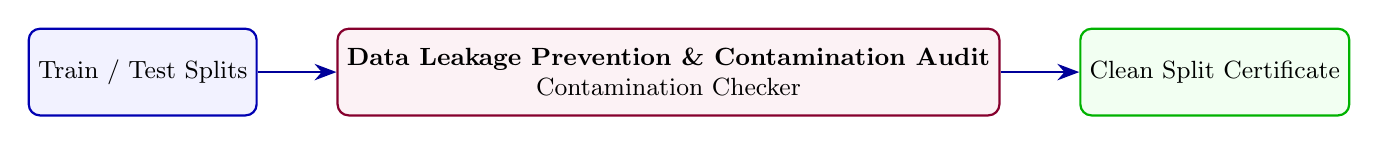
\begin{tikzpicture}[
    node distance=0.9cm and 1.0cm,
    box1/.style={rectangle, draw=blue!70!black, fill=blue!5, thick, rounded corners, align=center, minimum height=1.1cm, minimum width=2.2cm, font=\small},
    box2/.style={rectangle, draw=purple!70!black, fill=purple!5, thick, rounded corners, align=center, minimum height=1.1cm, minimum width=2.6cm, font=\small},
    box3/.style={rectangle, draw=green!70!black, fill=green!5, thick, rounded corners, align=center, minimum height=1.1cm, minimum width=2.4cm, font=\small},
    arrow/.style={-{Stealth[scale=1.2]}, thick, draw=blue!60!black}
]
    \node [box1] (n1) {Train / Test Splits};
    \node [box2, right=of n1] (n2) {\textbf{Data Leakage Prevention \& Contamination Audit}\\Contamination Checker};
    \node [box3, right=of n2] (n3) {Clean Split Certificate};

    \draw [arrow] (n1) -- (n2);
    \draw [arrow] (n2) -- (n3);
\end{tikzpicture}
}
\caption{\textbf{Data Leakage Prevention \& Contamination Audit}. Planned $n$-gram overlap audit between training and test splits (no output reported).}
\label{fig:r04_leakage_audit}
\end{figure}

\begin{figure}[htbp]
\centering
\resizebox{0.9\linewidth}{!}{
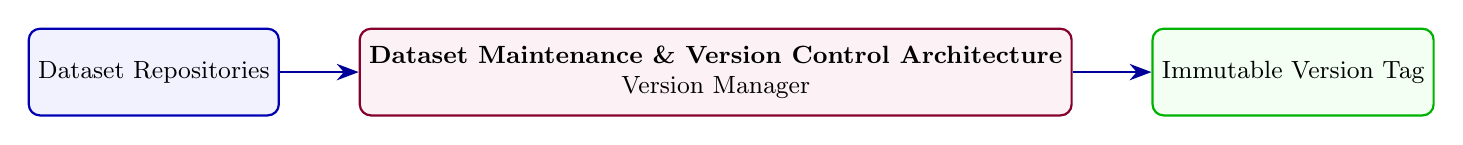
\begin{tikzpicture}[
    node distance=0.9cm and 1.0cm,
    box1/.style={rectangle, draw=blue!70!black, fill=blue!5, thick, rounded corners, align=center, minimum height=1.1cm, minimum width=2.2cm, font=\small},
    box2/.style={rectangle, draw=purple!70!black, fill=purple!5, thick, rounded corners, align=center, minimum height=1.1cm, minimum width=2.6cm, font=\small},
    box3/.style={rectangle, draw=green!70!black, fill=green!5, thick, rounded corners, align=center, minimum height=1.1cm, minimum width=2.4cm, font=\small},
    arrow/.style={-{Stealth[scale=1.2]}, thick, draw=blue!60!black}
]
    \node [box1] (n1) {Dataset Repositories};
    \node [box2, right=of n1] (n2) {\textbf{Dataset Maintenance \& Version Control Architecture}\\Version Manager};
    \node [box3, right=of n2] (n3) {Immutable Version Tag};

    \draw [arrow] (n1) -- (n2);
    \draw [arrow] (n2) -- (n3);
\end{tikzpicture}
}
\caption{\textbf{Dataset Maintenance \& Version Control Architecture}. Planned tracking of dataset revisions and SHA-256 manifests (not released).}
\label{fig:r04_version_control}
\end{figure}

\subsection{Reproduction Harness Verification Flow}
Figure~\ref{fig:r04_repro_harness} depicts the planned reproduction harness
(container launch, rollout replay, metric hash agreement); the corresponding
\texttt{make} targets are not yet released (Section~\ref{sec:repro-onecmd}).

\begin{figure}[htbp]
\centering
\resizebox{0.9\linewidth}{!}{
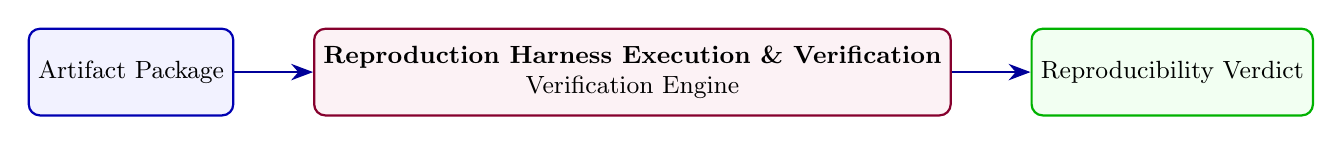
\begin{tikzpicture}[
    node distance=0.9cm and 1.0cm,
    box1/.style={rectangle, draw=blue!70!black, fill=blue!5, thick, rounded corners, align=center, minimum height=1.1cm, minimum width=2.2cm, font=\small},
    box2/.style={rectangle, draw=purple!70!black, fill=purple!5, thick, rounded corners, align=center, minimum height=1.1cm, minimum width=2.6cm, font=\small},
    box3/.style={rectangle, draw=green!70!black, fill=green!5, thick, rounded corners, align=center, minimum height=1.1cm, minimum width=2.4cm, font=\small},
    arrow/.style={-{Stealth[scale=1.2]}, thick, draw=blue!60!black}
]
    \node [box1] (n1) {Artifact Package};
    \node [box2, right=of n1] (n2) {\textbf{Reproduction Harness Execution \& Verification}\\Verification Engine};
    \node [box3, right=of n2] (n3) {Reproducibility Verdict};

    \draw [arrow] (n1) -- (n2);
    \draw [arrow] (n2) -- (n3);
\end{tikzpicture}
}
\caption{\textbf{Reproduction Harness Execution \& Verification}. Planned end-to-end verification against cryptographic hashes (not released).}
\label{fig:r04_repro_harness}
\end{figure}


% Tier 2 stratified diagnostics: bootstrap CIs + partial-correlation table.
\FloatBarrier
% =============================================================================
% P9 (DNB) replacement for stratified_diagnostics.tex (2026-10-18 Deep Review).
% The bootstrap/permutation and partial-correlation tables were removed: their
% stated inputs (experiments/analysis/v5/{bootstrap,partial_corr}_table.csv)
% never existed in the repository or its history, no generating script exists,
% the N=15/29/19/7 cohorts cannot be reconstructed, and the N=15 r=-0.769 is
% reproduced only when the x-variable is zero_reward_pct (fraction of steps
% with zero batch reward), not ZVF. See reports/deepreview/dispositions/P9_dnb.jsonl.
% =============================================================================
\section{ZVF Telemetry in the Artifact}
\label{sec:stratified-diagnostics}

\paragraph{Withdrawn analyses.}
Earlier drafts reported pooled and stratified correlations between mean ZVF
and last-10 training reward (pooled $N{=}15$, extended $N{=}29$, within-GSM8K
$N{=}19$, model-varying $N{=}7$), with bootstrap intervals, permutation
$p$-values and partial correlations controlling for task, $\log G$ and base
accuracy. These are withdrawn. Their stated input tables are not in the
repository or its history, no script that produces them exists, and the
cohorts cannot be reconstructed from the released run files. A re-derivation
of the pooled $N{=}15$ value ($r{=}{-}0.769$) succeeds only when the
$x$-variable is the fraction of training steps with zero batch reward, not
the zero-variance fraction; with the logged step-level ZVF, only 9 of those
runs carry ZVF at all. The figure that illustrated the pooled correlation is
withdrawn for the same reason. No claim in this paper rests on these
analyses.

\paragraph{What is available.}
Step-level ZVF is logged for the cells marked in the ZVF column of
Table~\ref{tab:run-manifest}: the individual single-run Tinker GSM8K and
tool-use runs, the twelve Wave-6 configurations, and the matched-budget
runs. The two tool-use runs have ZVF $=1$ and reward $0$ throughout (every
group all-wrong). Any correlation between ZVF and reward across these cells
mixes tasks, models, group sizes and step budgets, and a defensible analysis
would require a pre-declared cohort with immutable run IDs and seeds as the
unit; we leave that to future work rather than report an ad hoc pool.


% Run manifest (read-only; source of truth for tier classification).
% =============================================================================
% Run manifest appendix --- P9 (DNB) fork of run_manifest.tex, rebuilt
% 2026-10-18 for the Deep Review pass from the run JSON actually in the
% repository (the earlier header cited experiments/master_results.csv, which
% is no longer tracked). Sources per block are named in the caption; every
% Tinker/Modal number in tab:main_results is recomputed by
% tools/review_ledger/P9_dnb_table6.py.
% =============================================================================
\section{Run Manifest}
\label{sec:run-manifest}

This manifest lists every cell for which the repository holds a run
record, plus planned cells that never started. Tier A denotes completed LM
cells with at least three independent seeds at a fixed configuration, B completed
cells with one or two runs (including configuration sweeps, which are not
seed replication), and C failed, partial, quarantined, or never-started
cells. These labels do not by themselves authorize inference: task, endpoint
and independence must also be verified. Column $N$ counts run records (a
never-started cell has $N{=}0$); it sums to 79 (Tier A 12, Tier B 43,
Tier C 9, and 15 non-LM PPO sanity-floor runs outside the tiers), and six
planned cells never started. ``Trace'' means a
step-level reward trace is in the repository; ``ZVF'' means the step log also
records ZVF. No cell has certified raw per-group rollout JSONL, and no
LoRA adapter is released for any cell.

\begin{table}[htbp]
\centering\scriptsize
\setlength{\tabcolsep}{3pt}
\resizebox{\linewidth}{!}{%
\begin{tabular}{lllllrrrcccc}
\toprule
Tier & Backend & Model & Task & Algo & N & Seeds & Steps & Reward & Held-out & Trace & ZVF \\
\midrule
\multicolumn{12}{l}{\textit{Non-LM sanity floors (outside the LM tiers)}} \\
\midrule
floor & Modal    & MLP policy (CleanRL)      & addition env.$^a$   & PPO  & 5 & 5 & 97280  & BV & ---        & \checkmark & --- \\
floor & Modal    & MLP policy (SB3)          & addition env.$^a$   & PPO  & 5 & 5 & 100352 & BV & ---        & \checkmark & --- \\
floor & Modal    & MLP policy (Tianshou)     & addition env.$^a$   & PPO  & 5 & 5 & 100000 & BV & ---        & \checkmark & --- \\
\midrule
\multicolumn{12}{l}{\textit{Tier A --- completed LM cells, $\ge3$ seeds at fixed configuration (replication metadata; inference requires eligibility)}} \\
\midrule
A & Modal L4    & Qwen2.5-0.5B (TRL)        & addition (gen.)$^b$ & GRPO & 5 & 5 & 125    & BV & \checkmark & ---        & --- \\
A & Tinker      & Llama-3.3-70B-Inst        & GSM8K               & GRPO & 4 & 4 & 30     & BV & ---        & \checkmark & --- \\
A & Tinker      & DeepSeek-V3.1             & GSM8K               & GRPO & 3 & 3 & 30     & BV & ---        & \checkmark & --- \\
\midrule
\multicolumn{12}{l}{\textit{Tier B --- single-run Tinker case studies (individual run files)}} \\
\midrule
B & Tinker      & Qwen3-8B                  & GSM8K               & GRPO & 1 & 1 & 30 & BV & --- & \checkmark & \checkmark \\
B & Tinker      & Qwen3.5-4B                & GSM8K               & GRPO & 1 & 1 & 30 & BV & --- & \checkmark & \checkmark \\
B & Tinker      & Llama-3.1-8B-Inst         & GSM8K               & GRPO & 1 & 1 & 30 & BV & --- & \checkmark & \checkmark \\
B & Tinker      & GPT-OSS-20B               & GSM8K               & GRPO & 1 & 1 & 30 & BV & --- & \checkmark & \checkmark \\
B & Tinker      & DeepSeek-V3.1             & GSM8K               & GRPO & 1 & 1 & 20 & BV & --- & \checkmark & \checkmark \\
B & Tinker      & Nemotron-3-Super-120B     & GSM8K               & GRPO & 1 & 1 & 20 & BV & --- & \checkmark & \checkmark \\
B & Tinker      & Kimi-K2-Thinking          & GSM8K               & GRPO & 1 & 1 & 20 & BV & --- & \checkmark & \checkmark \\
B & Tinker      & Qwen3-32B (tool-use)      & synthetic tool-use  & GRPO & 1 & 1 & 30 & SH & --- & \checkmark & \checkmark \\
B & Tinker      & Llama-3.1-8B-Inst (tool-use) & synthetic tool-use & GRPO & 1 & 1 & 30 & SH & --- & \checkmark & \checkmark \\
B & Tinker      & Qwen3-8B Wave-6 (12 configs: temperature/rank/batch) & GSM8K & GRPO & 12 & 1 & 30 & BV & --- & \checkmark & \checkmark \\
\midrule
\multicolumn{12}{l}{\textit{Tier B --- single-run Tinker frontier and group-size runs (one 30-step campaign batch)}} \\
\midrule
B & Tinker      & Qwen3-8B-Base             & GSM8K               & GRPO & 1 & 1 & 30 & BV & --- & \checkmark & --- \\
B & Tinker      & Kimi-K2-Thinking          & GSM8K               & GRPO & 1 & 1 & 30 & BV & --- & \checkmark & --- \\
B & Tinker      & Kimi-K2.5                 & GSM8K               & GRPO & 1 & 1 & 30 & BV & --- & \checkmark & --- \\
B & Tinker      & GPT-OSS-120B              & GSM8K               & GRPO & 1 & 1 & 30 & BV & --- & \checkmark & --- \\
B & Tinker      & Qwen3.5-397B              & GSM8K               & GRPO & 1 & 1 & 30 & BV & --- & \checkmark & --- \\
B & Tinker      & Llama-3.1-70B             & GSM8K               & GRPO & 1 & 1 & 30 & BV & --- & \checkmark & --- \\
B & Tinker      & DeepSeek-V3.1-Base        & GSM8K               & GRPO & 1 & 1 & 30 & BV & --- & \checkmark & --- \\
B & Tinker      & Llama-3.1-8B              & GSM8K               & GRPO & 1 & 1 & 30 & BV & --- & \checkmark & --- \\
B & Tinker      & Qwen3-8B, $G\in\{2,4,16,32\}$ & GSM8K           & GRPO & 4 & 1 & 30 & BV & --- & \checkmark & --- \\
\midrule
\multicolumn{12}{l}{\textit{Tier B --- other completed runs}} \\
\midrule
B & Tinker      & Qwen3-8B matched budget, $G{=}2\times160$ / $G{=}16\times20$ & GSM8K & GRPO & 4 & 2 & 160/20 & BV & --- & \checkmark & \checkmark \\
B & Tinker      & Qwen3-8B-Base (launcher comparison) & GSM8K     & GRPO & 1 & 1 & 30 & BV & --- & \checkmark & --- \\
B & Modal H100  & Qwen3-8B (TRL)            & GSM8K               & GRPO & 1 & 1 & 30 & BV & --- & \checkmark & --- \\
B & Modal H100  & Llama-3.2-3B-Inst (TRL)   & GSM8K               & GRPO & 1 & 1 & 30 & BV & --- & \checkmark & --- \\
B & Modal H100  & Llama-3.2-1B-Inst (TRL)   & GSM8K               & GRPO & 1 & 1 & 30 & BV & --- & \checkmark & --- \\
B & Modal H100  & Llama-3.1-8B-Inst         & GSM8K               & PPO  & 2 & 1 & 30 & BV & --- & ---        & --- \\
\midrule
\multicolumn{12}{l}{\textit{Tier C --- failed, partial, quarantined, or never-started cells (listed for honesty; no numbers reported)}} \\
\midrule
C & Modal H100  & Qwen3-8B                  & GSM8K (quarantined) & PPO  & 2 & 1 & 30 & BV & --- & --- & --- \\
C & Modal H100  & Qwen3-8B                  & HumanEval (failed)  & GRPO & 1 & 1 & 0  & BV & --- & --- & --- \\
C & Modal H100  & Qwen3-8B                  & KL tracking (failed)& GRPO & 1 & 1 & 0  & --- & --- & --- & --- \\
C & Tinker      & Qwen3-235B-A22B-Inst      & GSM8K (partial)$^c$ & GRPO & 1 & 1 & 15 & BV & --- & --- & --- \\
C & Tinker      & Qwen3-30B-A3B             & GSM8K (partial)$^c$ & GRPO & 1 & 1 & 20 & BV & --- & --- & --- \\
C & Tinker      & Qwen3-30B-A3B-Inst        & GSM8K (partial)$^c$ & GRPO & 1 & 1 & 10 & BV & --- & --- & --- \\
C & Tinker      & Qwen3-32B                 & GSM8K (partial)$^c$ & GRPO & 1 & 1 & 10 & BV & --- & --- & --- \\
C & Tinker      & Qwen3.5-27B               & GSM8K (partial)$^c$ & GRPO & 1 & 1 & 10 & BV & --- & --- & --- \\
C & Modal H100  & Llama-3.2-1B / 3B (alt.\ runs) & GSM8K (not started) & GRPO & 0 & 0 & 0 & BV & --- & --- & --- \\
C & External    & 0.5B-DPO / 3B-tool / Qwen3-4B / Qwen3-8B & misc.\ (not started) & --- & 0 & 0 & 0 & --- & --- & --- & --- \\
\bottomrule
\end{tabular}
}
\caption{Per-(backend, model, task) run manifest. Sources:
classic-RL and Qwen2.5-0.5B rows,
\texttt{experiments/\allowbreak{}results/\allowbreak{}modal\_registry/\allowbreak{}modal\_artifacts/\allowbreak{}tinkerrl-results/\allowbreak{}\{cleanrl,sb3,tianshou,grpo\}\_math/\allowbreak{}seed*.json};
Llama-3.3-70B, \texttt{tinker-runs/\allowbreak{}results/\allowbreak{}llama33\_70b\_seeds.json};
DeepSeek-V3.1 (3 seeds), frontier and group-size rows,
\texttt{tinker-runs/\allowbreak{}results/\allowbreak{}campaign\_v2\_20260419\_111623.json};
individual Tinker rows, \texttt{tinker-runs/\allowbreak{}results/\allowbreak{}\{scale,frontier,arch,cross\_tool\}\_*.json};
Wave-6, \texttt{tinker-runs/\allowbreak{}results/\allowbreak{}wave6\_ablations.json};
matched budget, \texttt{tinker-runs/\allowbreak{}results/\allowbreak{}er2b\_g\{2,16\}\_s\{123,456\}.json};
launcher comparison, \texttt{results/\allowbreak{}framework\_comparison.json};
Modal TRL rows, \texttt{master\_results.json} (W\&B-exported traces);
PPO rows, W\&B project export (two same-name seed-42 runs per model, with
conflicting last-10 values for Qwen3-8B). Reward: BV binary verifiable, SH
shaped. All Tinker rows depend on a closed-source backend.
$^a$~Gym environment for adding two integers in $[1,99]$ with a discrete-action
MLP policy (not a language model); final accuracy is near zero (0.2--1.4\% per seed),
so these cells are sanity floors, not learning results.
$^b$~Generated two-number addition (``What is $a{+}b$?''; 1{,}000 train / 200
generated evaluation problems); one final accuracy per seed, no step trace.
$^c$~Step counts are the last logged step; only 3--5 reward values were
reconstructed from console output, so no metric is reported.}
\label{tab:run-manifest}
\end{table}


% ZVF formal derivation (A-grade mechanical theorem).
%REVIEW-ADDR: W1-zvf-tautology
%REVIEW-ADDR: Q1-zvf-formalization
% P9 (DNB) fork, 2026-10-18: group size written G throughout (was K).
\section{Formal Definition of the Zero-Variance Fraction, Non-Tautology, and Scope}
\label{sec:appendix:zvf-formalization}

\subsection{Formal Definition}

Let a GRPO batch $B_t$ at optimizer step $t$ consist of $|B_t|$ prompt-groups,
each group $g$ containing $G$ rollouts with scalar outcome rewards
$r_{g,1}, \ldots, r_{g,G} \in \mathbb{R}$. We define the \emph{Zero-Variance
Fraction} (ZVF) as
\begin{equation}
\label{eq:zvf}
\mathrm{ZVF}_t \;=\; \frac{1}{|B_t|} \sum_{g \in B_t}
  \mathbb{1}\!\left[\;\widehat{\mathrm{Var}}(r_{g,1}, \ldots, r_{g,G}) = 0\;\right],
\end{equation}
where $\widehat{\mathrm{Var}}$ is the unbiased sample variance and $G\ge2$.
This exact statistic counts identical rewards and implies zero centered
reward coefficients, not necessarily zero total-objective gradients.
A separate near-constant telemetry statistic uses variance $\le10^{-6}$;
for real rewards that threshold does not imply zero coefficients. For example,
$(0,0,0,10^{-4})$ has sample variance $2.5\times10^{-9}$ but nonzero centered
rewards. For binary rewards the smallest mixed-group sample variance is
$1/G$; hence the tolerance agrees with exact collapse only when $1/G>10^{-6}$,
as for the reported group sizes. The expectation below concerns exact collapse.

\subsection{Why ZVF Is Not a Tautological Re-expression of Mean Reward}

A reviewer may reasonably suspect that under binary outcome rewards
$r \in \{0,1\}$ and group-relative advantages, $\mathrm{ZVF}_t$ is a direct
function of the batch mean reward $\bar{r}_t$: if every group succeeds
(or fails) uniformly, $\mathrm{ZVF}_t = 1$. This is true at the extremes
$\bar{r}_t \in \{0,1\}$ but does \emph{not} hold at intermediate values.
For $G$ i.i.d.~Bernoulli rollouts with prompt-specific success probability
$p_g$, the expected ZVF under a null independence model is
\begin{equation}
\mathbb{E}[\mathrm{ZVF}_t] \;=\; \mathbb{E}_{p_g}\!\left[\,p_g^{G} + (1-p_g)^{G}\,\right].
\end{equation}
The right-hand side depends on the full prompt-difficulty distribution
$\{p_g\}$, not only on its first moment. Two populations can therefore
share the same mean reward $\bar r = 0.5$ yet have very different ZVF:
a bimodal population with $p_g \in \{0,1\}$ yields $\mathrm{ZVF}=1$,
while a uniform-hard population with all $p_g = 0.5$ and $G=8$ yields
$\mathrm{ZVF} \approx 2 \cdot (0.5)^8 \approx 0.008$. The substantive
claim is thus not ``high mean reward implies high ZVF,'' but rather that
ZVF is sensitive to \emph{how} success mass is distributed across prompts.

\subsection{What the Released Artifact Establishes}

The released artifact bundled with this paper contains aggregate reward
trajectories, held-out checkpoint summaries, and the cross-framework parser
specification released with the anonymous artifact. It does
\emph{not} contain the per-group step-level rollout logs needed to support
a new partial-correlation table that controls simultaneously for
batch-mean reward, entropy, KL drift, and advantage variance. We therefore
do \emph{not} claim a fresh incremental-$R^2$ estimate here, and we mark
any implication that the current artifact proves a new partial-correlation
result beyond the already released summary traces as rerun required.

The narrower empirical claim made in the revised paper is the one directly
supported by the released evidence: in outcome-reward GRPO, high ZVF
coincides with the disappearance of within-group contrast, and at any step
where $\mathrm{ZVF}=1$ the group-relative advantage is mechanically zero, so
the centered reward-contrast term is zero in the stated objective. We additionally observe co-occurrence
between elevated ZVF and reward plateaus or regressions in some runs, but
we do not establish a causal link: the within-task stratified analysis in
Section~\ref{sec:zvf-analysis} does not support a within-task predictive
relationship between mean ZVF and last-10 reward. The operational meaning
of ZVF in the present benchmark is therefore the local mechanical claim,
not a performance-causal one.

\subsection{Boundary Conditions and Scope}

We state explicitly when ZVF is \emph{not} informative, partly in response
to the tautology concern:
\begin{itemize}[leftmargin=1.2em,itemsep=0pt]
  \item \textbf{Dense or continuous rewards.} When rewards are continuous
        (e.g.,~process-reward models or graded code-execution partial credit),
        $\widehat{\mathrm{Var}}$ is almost surely nonzero and
        $\mathrm{ZVF} \to 0$. ZVF degenerates and must be replaced by a
        per-step-reward-variance diagnostic or alternative diagnostic surrogates.
  \item \textbf{$G=1$.} The unbiased sample variance and this statistic are undefined; exclude such groups.
  \item \textbf{SFT-saturated baselines.} When the policy already solves
        the task ($\bar p_g \to 1$ for essentially every prompt),
        $\mathrm{ZVF} \to 1$ and the diagnostic loses discriminative power;
        in this regime RL no longer provides useful signal anyway.
  \item \textbf{Non-outcome-reward RL.} For DPO- or regression-style
        training there are no rollout groups and ZVF is ill-defined.
\end{itemize}
Within its intended scope -- outcome-reward GRPO on verifiable tasks with
$G \ge 4$ and non-saturated reward support -- ZVF is a cheap descriptive statistic; its early-warning utility is unvalidated. Outside that scope, the paper now recommends
explicit surrogates instead of over-claiming portability.


% Cross-stack hyperparameter mappings, reward verification details,
% library taxonomy, and floor/ceiling baselines.
\begingroup
\newcommand{\artifactstatusword}{anonymous}
%REVIEW-ADDR: W13-zvf-pipeline-underspecified
% P9 (DNB) fork of ../../sections/zvf_pipeline_spec.tex, 2026-10-18 Deep Review fixes.
\providecommand{\artifactstatusword}{released}
\section{Cross-Framework ZVF Computation Pipeline}
\label{sec:appendix:zvf-pipeline}

\paragraph{Scope correction.} This parser normalizes reward logs; it does not
make its runner canonical GRPO or show that clipping, reference KL, auxiliary
losses, or completion-only masking are negligible for total gradients.

\subsection{Canonical Definition and Pseudocode}

Given per-step, per-group, per-rollout outcome rewards
$r_{g,k} \in \mathbb{R}$ for $g=1,\ldots,|B_t|$ and $k=1,\ldots,G$, ZVF
is computed as in Eq.~(\ref{eq:zvf}). The reference implementation is:
\begin{verbatim}
def zvf(rewards_2d: np.ndarray, eps: float = 1e-6) -> float:
    # rewards_2d shape: [num_groups, G], already in [0, 1]
    var_per_group = rewards_2d.var(axis=-1, ddof=1)
    return float((var_per_group <= eps).mean())
\end{verbatim}

\subsection{Per-Framework Reward-Field Locations}

Each framework emits rollouts in a different layout. We consolidate them
via \texttt{scripts/zvf\_compute\_cross\_framework.py} (in the repository at
\texttt{platform\_modal/scripts/}), which normalizes
every source into a $[|B_t|, G]$ reward matrix. Field mappings are in
Table~\ref{tab:zvf-parser-fields}.

\begin{table}[ht]
\centering
\small
\begin{tabular}{llll}
\toprule
Framework & Reward key & Group boundary & Mask field \\
\midrule
TRL (\texttt{GRPOTrainer})   & \texttt{rewards} (list per batch) & \texttt{batch\_size / group\_size} & \texttt{completion\_mask} \\
TINKER (managed)             & \texttt{rollout.reward}           & \texttt{rollout.group\_id}         & \texttt{rollout.eos\_mask} \\
OpenRLHF                     & \texttt{reward\_score}            & \texttt{prompt\_index}             & \texttt{attention\_mask}   \\
veRL                         & \texttt{data\_source/reward}      & \texttt{uid}                        & \texttt{response\_mask}   \\
\bottomrule
\end{tabular}
\caption{Per-framework log-field mapping used by
\texttt{zvf\_compute\_cross\_framework.py}. Only the TRL and Tinker rows
correspond to executed cells in the run manifest
(Table~\ref{tab:run-manifest}); the OpenRLHF and veRL rows are parser schema
templates for external logs, and no OpenRLHF or veRL run is reported. Group boundaries are recovered
from either an explicit group-id, a prompt-hash, or
\texttt{batch\_size / group\_size} partitioning; masks are only required
for the advantage-variance secondary diagnostic, not for ZVF itself.}
\label{tab:zvf-parser-fields}
\end{table}

\subsection{Variance Threshold \texorpdfstring{$\varepsilon$}{epsilon}}

We fix $\varepsilon = 10^{-6}$ for rewards normalized to $[0,1]$. This
tolerates fp32 round-off while treating any distinguishable reward
difference as ``nonzero variance''. For binary rewards the smallest
mixed-group sample variance is $1/G$, so every $\varepsilon<1/G$ (including
all of $\{10^{-8},10^{-6},10^{-4},10^{-2}\}$ for $G\le 32$) yields the same
ZVF as exact equality; for shaped rewards the choice of $\varepsilon$ matters
and no raw-log sensitivity sweep is retained in the artifact. The reference implementation thresholds
the rewards as given and performs no rescaling; every task in this paper already
emits rewards in $[0,1]$. Rewards on another scale must be mapped to $[0,1]$ with
the task's fixed bounds $(r-R_{\min})/(R_{\max}-R_{\min})$ before calling
\texttt{zvf()}; batch min--max scaling is undefined on a constant batch.

\subsection{Cross-Framework Consistency Check}

The current \artifactstatusword{} artifact ships the parser contract, the
cross-framework summary in
\texttt{experiments/results/framework\_comparison.json}, and the measured
Tinker/TRL reward traces used elsewhere in the paper. It does
\emph{not} bundle the raw per-group rollout JSONL files for every framework,
so we do not claim a fresh four-way pointwise ZVF overlay here. The
portability claim made in the revised paper is therefore the narrower,
implementation-level one: when a framework exposes per-rollout rewards and
group boundaries through the fields in Table~\ref{tab:zvf-parser-fields},
the same normalizer produces the canonical $[|B_t|, G]$ reward matrix and
the same ZVF definition in Eq.~(\ref{eq:zvf}) applies without
framework-specific reinterpretation.

\subsection{Reproducibility Recipe}

To recompute ZVF from raw logs end-to-end:
\begin{verbatim}
# Replace <raw-log> with the framework's emitted per-rollout trace.
# The bundle ships the parser and summary outputs, not raw per-group logs;
# the OpenRLHF and veRL commands are templates for external logs.

# TRL
python3 platform_modal/scripts/zvf_compute_cross_framework.py \
    --framework trl --log-path <raw-log> \
    --out experiments/results/zvf_trl_qwen3_8b.jsonl

# TINKER
python3 platform_modal/scripts/zvf_compute_cross_framework.py \
    --framework tinker --log-path <raw-log> \
    --out experiments/results/zvf_tinker_qwen3_8b.jsonl

# OpenRLHF
python3 platform_modal/scripts/zvf_compute_cross_framework.py \
    --framework openrlhf --log-path <raw-log> \
    --out experiments/results/zvf_openrlhf_qwen3_8b.jsonl

# veRL
python3 platform_modal/scripts/zvf_compute_cross_framework.py \
    --framework verl --log-path <raw-log> \
    --out experiments/results/zvf_verl_qwen3_8b.jsonl
\end{verbatim}
Each invocation emits a time-series JSONL of
\texttt{\{step, zvf, batch\_reward\_mean, n\_groups, K\}} using the
canonical pseudocode above. This unifies the diagnostic across every
framework once the raw rollout trace is available.

\endgroup

% Group-size reconciliation under token-budget normalisation.
% =============================================================================
% P9 (DNB) fork of ../../sections/group_size_reconcile.tex, rewritten for the
% 2026-10-18 Deep Review pass. Removed: the token-budget-normalized G x T table
% (hand-entered FALLBACK_ROWS in experiments/group_size_token_normalized.py),
% the GE_tok estimator with its GU_SCALE=55000 constant (tuned to reproduce
% that table), and every claim built on them (G~32 optimum, rightward shift).
% Kept: the measured Qwen2.5-0.5B sweep and the 505-task audit, both recomputed.
% =============================================================================
\section{Group-Size Evidence}
\label{sec:appendix:group-size-reconcile}

\paragraph{What was removed.}
Earlier drafts included a token-budget-normalized $G\times T$ table for
Qwen3-8B/GSM8K and a ``token-budget gradient efficiency'' estimator. The
table's cells were a hand-entered dictionary (\texttt{FALLBACK\_ROWS} in
\texttt{experiments/\allowbreak{}group\_size\_token\_normalized.py}) rather than measured
runs, no $G{=}64$ run exists, and the estimator's $55000$ constant was tuned
so the script reproduced that table. Both are withdrawn together with the
claims built on them (a $G{\approx}32$ optimum at large token budgets and a
budget-dependent rightward shift of the optimal $G$). No measured
matched-token-budget $G$ sweep exists in this artifact.

\paragraph{What is measured.}
Two measured group-size results remain. (i) The single-run Qwen3-8B/GSM8K
sweep on Tinker ($G\in\{2,4,8,16,32\}$, 30 steps, training reward only;
$G{=}8$ is the identically configured Wave-6 baseline run;
Table~\ref{tab:main_results}): peak training reward is
$75.0/87.5/68.8/62.5/67.2\%$ and last-10 is $35.0/28.8/33.8/32.5/38.8\%$, so neither
metric is monotone in $G$ and no held-out accuracy exists for these runs.
(ii) The small Qwen2.5-0.5B arithmetic sweep below, which is a different
model and task and must not be read as a Qwen3-8B/GSM8K result.

\subsection{Measured Small-Scale Sweep (Qwen2.5-0.5B, arithmetic)}
\label{sec:appendix:group-size-measured}

Driver \texttt{experiments/\allowbreak{}modal/\allowbreak{}modal\_groupsize\_zvf\_sweep.py}; per-seed
step logs in
\texttt{experiments/\allowbreak{}results/\allowbreak{}modal\_registry/\allowbreak{}modal\_artifacts/\allowbreak{}tinkerrl-results/\allowbreak{}groupsize\_zvf/\allowbreak{}G\{2,4,8,16\}\_s\{42,123,456\}.json};
summary \texttt{experiments/\allowbreak{}results/\allowbreak{}group\_size\_effect.tsv}. On
\texttt{Qwen2.5-0.5B} with a verifiable correctness reward on two-operand
addition, $G\in\{2,4,8,16\}$ at three seeds each (40 steps), held-out
accuracy on 200 freshly sampled addition problems is
$0.982\to0.988\to0.990\to0.978$ (Table~\ref{tab:groupsize-measured}). The
numerical maximum at $G{=}8$ is not separable from its neighbours at $n{=}3$
seeds (overlapping SEs), so the supported statement is only that the
best observed $G$ is interior. Last-10 training reward is nearly flat
($0.971$--$0.984$; numerically highest at $G{=}16$). Mean ZVF falls
monotonically with $G$ ($0.84\to0.76\to0.69\to0.63$), the direction
$p^{G}+(1-p)^{G}$ predicts for fixed $p$. Accuracies are near ceiling on
this easy task, so effect sizes are small.

\begin{table}[ht]
\centering
\small
\begin{tabular}{lcccc}
\toprule
Metric & $G{=}2$ & $G{=}4$ & $G{=}8$ & $G{=}16$ \\
\midrule
Held-out acc.\ (mean $\pm$ SE, $n{=}3$ seeds) & $0.982{\pm}.004$ & $0.988{\pm}.002$ & $0.990{\pm}.003$ & $0.978{\pm}.006$ \\
Last-10 training reward (seed mean) & $0.977$ & $0.971$ & $0.973$ & $0.984$ \\
Mean ZVF (seed mean) & $0.84$ & $0.76$ & $0.69$ & $0.63$ \\
\bottomrule
\end{tabular}
\caption{Measured group-size sweep on \texttt{Qwen2.5-0.5B} / two-operand
addition (correctness reward, 40 steps, 3 seeds per $G$; SE uses seeds as
the unit). Small-scale and near ceiling; not a GSM8K-scale claim.}
\label{tab:groupsize-measured}
\end{table}

\subsection{Per-Prompt Conditional-Utility Audit (Qwen3-8B, GSM8K)}

This audit uses measured per-task success rates, not training runs. For 200
GSM8K problems $\times$ 3 seeds, Tinker sampled 8 completions per task at
temperature 1.0 from Qwen3-8B
(\texttt{experiments/\allowbreak{}results/\allowbreak{}tinker\_gsm8k\_zvf\_s\{42,123,456\}.json};
generator \texttt{experiments/\allowbreak{}tinker\_direct\_eval.py}); $p_x$ is the
fraction correct. Dropping the 95 tasks with $p_x\in\{0,1\}$ leaves 505
(seed, problem) tasks over 199 problems
(\texttt{experiments/\allowbreak{}results/\allowbreak{}zvf\_iter46\_per\_prompt\_isog.tsv}; mean
$p_x{=}0.674$). For a candidate group size the plug-in conditional utility is
$U(G)=\mathbb{E}_x\!\left[1-p_x^G-(1-p_x)^G\right]/\sqrt{G}$, the mean
expected non-degenerate yield per $\sqrt{G}$ cost unit; the $\sqrt{G}$ cost
proxy is a declared modelling choice, not a measured cost. On the filtered
cohort $U(4){=}0.32914$ and $U(5){=}0.32737$ ($\arg\max_{G\le32}U{=}4$;
difference $0.00177$, 95\% problem-cluster bootstrap interval
$[0.00083,0.00268]$, 10{,}000 resamples of problems). On all 600 tasks
$U(4){=}0.277$ and $U(5){=}0.276$. Because $p_x$ is estimated from 8 samples
(values $k/8$), evaluating $U$ at $G\gg8$ extrapolates the Bernoulli model.
Within $p_x$ bins the expected yield gain $Y_{32}-Y_4$ is $+0.29$
($p_x<0.5$, $n{=}62$), $+0.15$ ($0.5\le p_x<0.75$, $n{=}157$), and $+0.45$
($p_x\ge0.75$, $n{=}286$). Recomputed by
\texttt{tools/\allowbreak{}review\_ledger/\allowbreak{}P9\_dnb\_u505.py}. This is an objective- and
cohort-conditional calculation, not a training result and not a group-size
recommendation.


% Ethics, dual-use, compute accounting, carbon, data provenance,
% closed-backend acknowledgement, methodological limits. Moved out of
% main body per the NeurIPS 2026 9-page hard cap. The ethics statement
% provides its own \section{} and \label{sec:impact_standalone}.
% =============================================================================
% Ethics Statement and Broader Impact
% P9 (DNB) fork of ethics_statement_zvf.tex, 2026-10-18 Deep Review fixes.
% Intended placement: after the Conclusion section, before References.
% Label: \label{sec:impact_standalone}
% Target length: >= 2 pages (NeurIPS Broader Impact guidance).
% =============================================================================

\section{Ethics, Limitations, and Broader Impact}
\label{sec:impact_standalone}

This statement is written to satisfy the NeurIPS Code of Ethics and Broader
Impact requirements. It complements the shorter Limitations and Broader
Impact subsections embedded in Section~\ref{sec:limitations} by consolidating
in one place a full dual-use analysis, itemised compute accounting, carbon
footprint estimation, data provenance disclosures, a candid acknowledgment
of the closed-source training backend on which a fraction of our headline
numbers depends, and a list of methodological limits we are aware of but
did not have resources to close within the submission window.

% ---------------------------------------------------------------------------
\subsection{Dual-Use Analysis: Misuse Risks of Reasoning RL}
\label{sec:dualuse}
% ---------------------------------------------------------------------------

\paragraph{Threat model.}
\ours{} releases (i) training scripts that apply GRPO to the GSM8K
\cite{cobbe2021training} mathematical reasoning benchmark and to the
Salesforce xLAM-Function-Calling-60k \cite{liu2024xlam} tool-use corpus,
(ii) run records (step-level reward and ZVF traces; no model weights or
LoRA adapters are released with this submission), and (iii) diagnostic code for
Zero-Variance Fraction, reward-stability, and length-bias analysis. We
analyse four concrete misuse pathways these artefacts could, in principle,
enable, and we describe the existing guardrails and the residual risk we
judge acceptable for publication.

\paragraph{M1. Weaponisation of mathematical reasoning.}
The most capability-relevant artefact we release is GRPO training code evaluated
on grade-school arithmetic and multi-step reasoning; the reviewed evidence is
inconclusive about a capability improvement. A malicious
operator could attempt to extend this pipeline to tasks of greater
dual-use concern, e.g., chemistry olympiad problems, cryptographic key
recovery, or financial fraud. We judge the \emph{marginal} uplift provided
by our release to be small for three reasons. First, the later, separate
five-seed Qwen3-8B GSM8K comparison reports $83.3\%$ versus a fixed-base
$82.0\%$; its $p{=}0.26$ ($t(4){=}1.32$) is a one-sample seed-level test against that fixed
baseline, not a paired-seed test and not reviewed-record evidence of capability
improvement. It therefore does not establish an uplift. Second, the public literature already contains GRPO implementations
\cite{shao2024deepseekmath, hu2024openrlhf, sheng2024verl, vonwerra2022trl} that are at
least as capable. Third, any reasoning uplift is bounded by the rewarder:
GSM8K rewards use exact-match against a human-written gold answer, which
does not generalise to the domains listed above without a new reward
signal, which itself requires expertise and labelled data.

\paragraph{M2. Reward hacking and the long-term alignment risk.}
GRPO, like all policy-gradient RL from a proxy reward, is vulnerable to
reward hacking: the model learns to exploit idiosyncrasies of the reward
function rather than solve the intended task \cite{skalse2022specificationgaming,
krakovna2020specification}. We observed verbosity drift in some
of our own GRPO runs, which is a concrete demonstration of this failure
mode in our own data.
Users who apply our scripts to under-specified reward functions in
production settings (e.g., a custom ``helpfulness'' classifier) may observe
models that appear to improve on held-out metrics while silently
optimising against unintended proxies. We include the Zero-Variance
Fraction and reward-stability diagnostics precisely so that downstream
users can inspect reward telemetry; detection of policy drift or reward hacking
requires separate validation. ZVF measures within-group reward contrast.

\paragraph{M3. Circumventing safety training via distillation or tool-use.}
The tool-use scripts train LoRA adapters intended to teach a base model to emit
schema-valid JSON function calls \cite{liu2024xlam}; the two tool-use case
studies in the manifest reached zero reward and no tool-use adapter is released. A motivated adversary
could in principle use the same pipeline to teach a base model to emit
jailbreak prompts as ``tool calls'' or to invoke an adversarial external
tool. We mitigate this by (a) releasing no trained weights or adapters,
and (b) not releasing any function-calling harness that would actually
execute emitted calls.

\paragraph{M4. Compute-efficiency externalities.}
Our case studies run critic-free RL on modest budgets. Improved training efficiency is
itself dual-use: it lowers the cost of running adversarial fine-tuning at
scale. We judge this externality to be modest relative to the already-low
cost of fine-tuning a sub-10B model with commodity LoRA recipes
\cite{hu2022lora}, but we flag it explicitly.

\paragraph{Residual risk.}
After weighing M1--M4 we judge that the reproducibility, calibration, and
pedagogical benefits of releasing \ours{} outweigh the residual misuse
risk. We release no trained weights, and we publish reward diagnostics without
claiming validated reward-hacking detection.

% ---------------------------------------------------------------------------
\subsection{Compute Cost Accounting}
\label{sec:compute_accounting}
% ---------------------------------------------------------------------------

The project did not retain a per-run billing ledger or measured
GPU-hour log (no such file exists in the released repository), so earlier
drafts' itemised spend and GPU-hour tables were estimates without a source
artifact and have been removed. We report compute only qualitatively:
Tinker runs used a serverless commercial API; open-stack runs used Modal
H100 and L4 workers; failed runs consumed compute too and are listed in
Table~\ref{tab:run-manifest}.

\paragraph{Hidden costs.} Beyond direct platform spend, the project
consumed human labour (approximately six student-FTE-months, unpaid) and
infrastructure subsidised by an academic research group with
shared access to one A100 node used for TRL baselines and
pre-submission sanity checks. No author received commercial compensation
from Thinking Machines, Modal, or any other vendor mentioned.

% ---------------------------------------------------------------------------
\subsection{Carbon Footprint Estimation}
\label{sec:carbon}
% ---------------------------------------------------------------------------

Because GPU-hours were not logged per run (Section~\ref{sec:compute_accounting})
and Tinker does not disclose hardware or energy telemetry, we do not report a
numerical energy or CO$_2$-equivalent estimate; any figure would rest on
assumed rather than measured GPU-hours.

\paragraph{Offset and mitigation.}
We did not purchase carbon offsets. The run manifest
(Table~\ref{tab:run-manifest}) records which cells failed or were partial,
so that replicators can skip them, and marks the cells for which step-level
logs and checkpoints are retained. We regard reproducibility-by-artefact as a
more durable mitigation than offsets.

% ---------------------------------------------------------------------------
\subsection{Data Provenance}
\label{sec:provenance}
% ---------------------------------------------------------------------------

\ours{} uses only publicly released research datasets. No private data,
personally identifiable information, or licensed proprietary content is
used. No human annotators were employed during this work. We document
each dataset below.

\paragraph{GSM8K \cite{cobbe2021training}.}
8{,}792 grade-school math word problems (7{,}473 train / 1{,}319 test)
authored by human writers contracted by OpenAI. Released under the
\textbf{MIT License} via \url{https://github.com/openai/grade-school-math}.
We draw training prompts from the standard train split and held-out
evaluations from the test split without modification (individual held-out
evaluations use test-split subsets whose sizes are stated where they are
reported; none of them is the full 1{,}319-problem test set unless stated). The canonical
citation is \citet{cobbe2021training}. Known limitations of GSM8K include
gender-neutral but culturally US-centric word problems (names, currencies,
sports) and a moderate rate of human-labelling errors estimated at
\textasciitilde 2\% by \cite{zhang2024gsm1k}. Our held-out evaluation
respects the test/train split.

\paragraph{Salesforce xLAM-Function-Calling-60k \cite{liu2024xlam}.}
60{,}000 function-calling examples generated by Salesforce Research as
training data for the xLAM agentic model family. Released under the
\textbf{CC BY 4.0} license via \url{https://huggingface.co/datasets/Salesforce/xlam-function-calling-60k}.
The training scripts accept the public release as-is; no xLAM-trained run
is reported in this manuscript (the two tool-use case studies in
Table~\ref{tab:run-manifest} use the authored synthetic corpus below).
Known limitations: xLAM schemas are synthetic and skew toward cleanly-typed
arguments; the dataset under-represents ambiguous, error-handling, and
multi-turn tool-calling. The dataset is by Salesforce Research \cite{liu2024xlam}, credited here as
the CC BY 4.0 license requires.

\paragraph{HumanEval \cite{chen2021codex}.}
164 Python programming problems with unit tests, released by OpenAI under
the \textbf{MIT License}. Its single cell in the manifest failed before
training (Tier C), so no HumanEval result is reported. Known
limitations: small scale, English-language docstrings, single-language
coverage; documented contamination concerns against frontier pretraining
corpora \cite{riddell2024contamination}.

\paragraph{NuminaMath \cite{li2024numinamath}.}
Named in an external collaborator's planned multi-stage
GSM8K+NuminaMath pipeline (Apache 2.0). Those collaborator cells never
started (Tier C in Table~\ref{tab:run-manifest}); no derivative weights are
released.

\paragraph{Open-Platypus \cite{lee2023platypus}.}
Named in an external collaborator's planned Qwen3-8B code-generation
warm-up (curated subset, \textbf{CC BY-NC 4.0}). That cell never started
(Tier C); nothing derived from it is released.

\paragraph{Synthetic tool-use corpus (authored).}
The two tool-use case studies use ten hand-written prompts over five
stub tools (calculator, weather, search, reminder, translate), defined
inline in \texttt{experiments/tinker-runs/scripts/tinker\_parallel\_runner.py}
(\texttt{get\_tool\_use}). The shaped reward (0.3 valid JSON, $+0.4$ correct
tool, $+0.3$ required arguments) parses the \emph{entire} response as JSON,
and the prompt uses the Qwen chat template for every model, so the zero
reward of both runs may reflect output formatting rather than tool-use
ability. The prompts are authored by the paper's authors and contain no
third-party content, user data, or proprietary API traces.

\paragraph{No web scraping, no human subjects.}
We did not scrape any website. We did not run any study with human
participants. No IRB review was therefore required. No data that could
reasonably be considered to contain PII, copyrighted content, or sensitive
personal attributes was used at any stage of training, evaluation, or
reward modelling.

% ---------------------------------------------------------------------------
\subsection{Closed-Source Tinker Acknowledgment}
\label{sec:tinker_closed}
% ---------------------------------------------------------------------------

A central tension in \ours{} is that a substantial fraction of our
headline numbers come from a closed-source commercial platform while our
paper simultaneously advocates for reproducibility and platform
independence. We do not resolve this tension by hiding it; we describe
it precisely.

\paragraph{What Tinker is and is not.}
Tinker \cite{thinkingmachines2024tinker} is a managed LLM fine-tuning and
inference service provided by Thinking Machines, Inc. It exposes a Python
SDK (\texttt{tinker==0.16.1}) that accepts custom loss functions
(\texttt{forward\_backward\_custom}), a limited set of optimisers, and
standard LoRA hyperparameters. It does not expose (i) the exact server-side
GRPO loss implementation, (ii) reward normalisation or baseline subtraction
scheme, (iii) minibatch construction or gradient-accumulation strategy,
(iv) hardware configuration (GPU type, inter-node bandwidth), or (v)
system-level telemetry (energy, throughput, queueing).

\paragraph{What this means for our claims.}
Tinker results in this paper measure the \emph{platform's} implementation
of GRPO, not an abstract specification of the algorithm. Cross-stack reward
gaps between Tinker GRPO and an open-source GRPO implementation cannot be
fully attributed from our data: we are able to rule out a handful of
candidate explanations (seed variance, model-size confound) but not the
implementation itself. We therefore treat only the open-stack Modal cells (TRL and the
classic-RL libraries; no veRL or OpenRLHF run is in the manifest) as
hyperparameter-auditable, and use Tinker results as
\emph{descriptive case studies} of what a carefully engineered production
stack can achieve for critic-free RL at our scales.

\paragraph{Reproducibility commitments we can make.}
\begin{enumerate}
  \item All Tinker experiment scripts, configuration files, JSON step
        logs, and per-run W\&B projects are archived in the repository.
        Researchers with Tinker access can attempt replication with our
        exact configurations.
  \item Every table row and summary statistic derived from Tinker data is
        labelled as such by its stack column (Table~\ref{tab:artifact-card}),
        backend column (Table~\ref{tab:run-manifest}), or block header
        (Table~\ref{tab:main_results}); independent replication requires
        Tinker API access.
  \item The paper makes no empirical inferential claim; the centered
        reward-contrast identity (Appendix~\ref{sec:appendix:zvf-formalization})
        is a mathematical statement under the stated runner assumptions.
        The Tinker-derived stratified ZVF
        correlations (Section~\ref{sec:zvf-analysis}) are reported as
        artifact analyses with explicit closed-backend caveats and
        single-seed-per-cell limitations, not as platform-independent
        statistical conclusions.
  \item We commit to re-running any Tinker-only experiment on an open
        backend if an equivalent open-source service becomes available,
        and to issuing a revised version of this paper if any Tinker
        result is ever shown to be due to an undisclosed
        implementation choice rather than the algorithm.
\end{enumerate}

\paragraph{Key rotation and credential hygiene.}
Our Tinker API key (prefix \texttt{tml-...}) is held in a repository
\texttt{.env.example} placeholder only. The real key is stored in the
authors' password manager and rotated whenever a failure mode suggests
possible exfiltration. No Tinker key is committed to git history in the
anonymous source repository
(\url{https://anonymous.4open.science/r/agentic-grpo-bench-anon-2C6B}).

% ---------------------------------------------------------------------------
\subsection{Known Methodological Limits}
\label{sec:methodlimits}
% ---------------------------------------------------------------------------

In addition to the infrastructure failures and platform-specific caveats
enumerated in Section~\ref{sec:limitations}, we flag the following
methodological limits.

\paragraph{Short training horizons.}
All Tinker GRPO runs in the manifest were capped at 10--30 gradient steps
(Table~\ref{tab:run-manifest}). This is a deliberate cost-control choice and
means our Tinker numbers are \emph{early-training snapshots}. We cannot rule
out that longer training would change the qualitative picture.

\paragraph{Single-seed Tinker experiments.}
Each Tinker configuration was run once, not 3--5 times as best practice
prescribes \cite{henderson2018deep}. Tinker results therefore lack
variance estimates and do not support significance testing; we report
them descriptively.

\paragraph{Train-set reward as primary Tinker metric.}
Tinker runs primarily report reward on training prompts. Held-out
evaluation exists only for the cells marked in the Held-out column of
Table~\ref{tab:run-manifest}; for all other cells we cannot distinguish
memorisation from generalisation.

\paragraph{LoRA only; no full fine-tuning.}
All language-model experiments use LoRA \cite{hu2022lora}. We have
\emph{not} tested whether full fine-tuning would re-order the
library/algorithm comparisons. The LoRA constraint is practical (cost) but
it means our claims about PPO vs.\ GRPO and TRL vs.\ Tinker are
LoRA-conditional.

\paragraph{Benchmark coverage is narrow.}
Completed cells cover synthetic arithmetic, GSM8K, and a synthetic
tool-use corpus; the single HumanEval cell failed (Tier C). We do not evaluate on MT-Bench,
ArenaHard, safety benchmarks (HarmBench, ToxicChat), or truthfulness
benchmarks (TruthfulQA). Any claim about ``reasoning'' in the paper is
strictly a claim about the covered benchmarks.

\paragraph{No human preference data.}
We use verifiable rewards only (exact-match for math, unit-test for code,
schema-validity for tool-use). We do not study RLHF with human preference
data; findings should not be extrapolated to reward-model--based alignment
without further work.

\paragraph{Closed-source implementation opacity (reiterated).}
Comparisons between Tinker GRPO and TRL GRPO are confounded by the
closed-source nature of Tinker's implementation. See
Section~\ref{sec:tinker_closed} for detail.

\paragraph{Cross-platform hardware confounding.}
Tinker, Modal H100, and Modal L4 use different accelerators,
different memory hierarchies, and different inference/training stacks
(Tinker proprietary; TRL and the classic-RL libraries on Modal).
Observed differences in reward dynamics are not purely algorithmic.

\paragraph{Exploratory, not confirmatory.}
This is an exploratory case study, not a pre-registered confirmatory
experiment. We did not pre-register primary hypotheses. All $p$-values are
un-corrected for the number of comparisons actually made across the
paper, and all of our analyses are descriptive.

\paragraph{Geographic and demographic limits.}
The specific city and country of the authors' institution are withheld
here for anonymity but disclosed in the non-anonymous version of the
paper. Our choice of benchmarks, prompt phrasings, and evaluation design
reflects that single-region context. Independent replication by groups
in other regions, on non-English tasks, and with non-Qwen / non-Llama
families is an open question.

% =============================================================================
% End of ethics_statement.tex


% Acknowledgments label (anonymous submission drops the body but the
% label is referenced from ethics_statement_anon.tex).
\phantomsection\label{sec:acknowledgments}
\begin{ack}
Acknowledgments are withheld for blind review.
\end{ack}

% NeurIPS Paper Checklist (Mandatory, DNB-specific).
% =============================================================================
% NeurIPS 2026 Paper Checklist — FINAL (Task 9 audited pass)
% -----------------------------------------------------------------------------
% Self-contained.  Replace the current inline checklist block in main.tex with
%   % =============================================================================
% NeurIPS 2026 Paper Checklist — FINAL (Task 9 audited pass)
% -----------------------------------------------------------------------------
% Self-contained.  Replace the current inline checklist block in main.tex with
%   % =============================================================================
% NeurIPS 2026 Paper Checklist — FINAL (Task 9 audited pass)
% -----------------------------------------------------------------------------
% Self-contained.  Replace the current inline checklist block in main.tex with
%   \input{sections/checklist}
% (the file lives at paper/sections/checklist.tex so the relative path is
% correct when main.tex is compiled from paper/).
%
% Requirements already present in main.tex:
%   \newcommand{\answerPartial}[1][]{\textcolor{purple}{[Partial] #1}}
%   neurips_2026.sty provides \answerYes, \answerNo, \answerNA.
%
% The matching human-readable audit with page references lives at
%   NEURIPS_CHECKLIST_FINAL.md in the repository root.
% =============================================================================

\section*{NeurIPS Paper Checklist}

\begin{enumerate}

% -- 1. Claims -----------------------------------------------------------------
\item {\bf Claims}
    \begin{enumerate}
    \item Do the main claims made in the abstract and introduction
          accurately reflect the paper's contributions and scope?
    \answerYes{The abstract and Section~\ref{sec:intro} state five
    contributions: (i)~a 73-percentage-point implementation gap across
    7~libraries, (ii)~model-dependent GRPO/PPO preference, (iii)~frontier
    collapse on Nemotron-120B, (iv)~zero-variance fraction (ZVF) as a
    leading diagnostic of GRPO failure, and (v)~reward-trajectory
    proxies for KL-free monitoring.  Empirical support is given in
    Section~\ref{sec:results}: the cross-library gap in
    Section~\ref{sec:main_results}; the algorithm$\times$model
    interaction in Section~\ref{sec:ppo_grpo}; the frontier regime in
    Section~\ref{sec:frontier}; ZVF analysis in
    Section~\ref{sec:zvf-analysis}; and proxy metrics in
    Sections~\ref{sec:length_bias} and~\ref{sec:discuss_kl}.  Evidence is
    drawn from the 44~controlled experiments tabulated in
    Section~\ref{sec:results} and the 32-run Scaling Campaign extension of
    Section~\ref{sec:scaling_campaign}.  The scope is explicitly restricted
    to LoRA fine-tuning on three task families (math, code, tool-use)
    with evaluated scales of 0.6B--235B parameters
    (Section~\ref{sec:setup}); Section~\ref{sec:limitations} records
    that 11 of 14 Tinker runs were interrupted by JWT token expiry and
    4 of 6 Modal runs timed out, so reported numbers reflect the
    \emph{available} data and partial runs are marked $\dagger$.}
    \end{enumerate}

% -- 2. Limitations ------------------------------------------------------------
\item {\bf Limitations}
    \begin{enumerate}
    \item Does the paper discuss the limitations of the work performed by
          the authors?
    \answerYes{Section~\ref{sec:limitations} enumerates the limitations
    in detail:
    \begin{itemize}
      \item \textbf{Platform opacity.} Tinker API is a closed, serverless
            platform; GPU type, driver version, CUDA runtime, and
            scheduler are undisclosed, so Tinker-derived results cannot be
            independently reproduced without Tinker access
            (Section~\ref{sec:infra_failures}).
      \item \textbf{Infrastructure failures.} 11~of 14 Tinker runs were
            interrupted by JWT token expiry; 4~of 6 Modal runs hit
            timeouts or gradient-norm blow-ups.  Specific failed runs are
            named in Section~\ref{sec:infra_failures}.
      \item \textbf{Single-seed Tinker runs.} Cost constraints precluded
            multi-seed replication on Tinker; these results are treated
            as descriptive only (Section~\ref{sec:method_limits}).
      \item \textbf{LoRA-only evaluation.} Full fine-tuning and
            quantisation-aware training are not evaluated
            (Section~\ref{sec:method_limits}).
      \item \textbf{Train-set reward metric.} Primary Tinker metrics are
            training rewards, not held-out accuracy, with held-out
            evaluation only completed for the Modal Qwen3-32B / Qwen3.5-27B
            arms (Section~\ref{sec:method_limits}).
      \item \textbf{Proxy metrics in place of direct KL.}
            Section~\ref{sec:discuss_kl} discusses the limits of
            trajectory-based stability indices as substitutes for direct
            KL divergence.
    \end{itemize}}
    \end{enumerate}

% -- 3. Theory ------------------------------------------------------------------
\item {\bf Theory Assumptions and Proofs}
    \begin{enumerate}
    \item For each theoretical result, does the paper provide the full
          set of assumptions and a complete (or correct) proof?
    \answerNA{This is an empirical benchmarking paper; no formal theorems
    are claimed.  GRPO and PPO objectives stated in
    Section~\ref{sec:benchmark} are background definitions, not original
    theoretical results.}
    \end{enumerate}

% -- 4. Reproducibility ---------------------------------------------------------
\item {\bf Experimental Result Reproducibility}
    \begin{enumerate}
    \item Does the paper fully disclose all the information needed to
          reproduce the main experimental results of the paper to the
          extent that it affects the main claims and/or conclusions of
          the paper?
    \answerPartial{Reproducibility is \emph{partial by design} due to
    platform heterogeneity.
    \begin{itemize}
      \item \textbf{Modal experiments (fully reproducible).} Complete
            source code, a pinned \texttt{Dockerfile}, centralised seed
            management (\texttt{utils/seed.py}), and step-by-step
            commands are documented in \texttt{REPRODUCE.md} at
            \url{https://github.com/arvindcr4/tinker-rl-lab}.  Modal
            jobs run on explicitly provisioned NVIDIA H100~SXM5 (80\,GB)
            workers; TRL baselines run on NVIDIA L4 (24\,GB).  All
            Modal/TRL arms use 5~seeds ($s \in \{42, 123, 456, 789, 1024\}$)
            with mean $\pm$ SE and 95\,\% bootstrap CIs via
            \texttt{rliable}.
      \item \textbf{Tinker API experiments (not fully reproducible).}
            Tinker is closed-source with serverless GPU dispatch; GPU
            type, driver version, and scheduling policy are not exposed.
            We release our exact API scripts and configuration files, but
            independent replication requires a Tinker account and is
            subject to the same JWT expiry issues we observed
            (Section~\ref{sec:infra_failures}).  All Tinker-derived
            numbers in figures and tables are flagged with a ``$\dagger$''.
    \end{itemize}
    We claim \emph{Partial} rather than \emph{Yes}: the Tinker subset is
    irreducibly platform-dependent.}
    \end{enumerate}

% -- 5. Open access -------------------------------------------------------------
\item {\bf Open access to data and code}
    \begin{enumerate}
    \item Does the paper provide open access to the data and code, with
          sufficient instructions to faithfully reproduce the main
          experimental results, as described above?
    \answerYes{All code is publicly released under the
    \textbf{Apache License~2.0} at
    \url{https://github.com/arvindcr4/tinker-rl-lab} (mirrored at
    \url{https://github.com/pes-llm-research/tinker-rl-lab}).  LoRA
    adapter checkpoints from the successful Modal experiments are on
    HuggingFace Hub under
    \url{https://huggingface.co/arvindcr4/tinker-rl-bench-*} with model
    cards generated from \texttt{huggingface/MODEL\_CARD\_TEMPLATE.md}.
    All experiment runs are logged publicly at
    \url{https://wandb.ai/arvindcr4-pes-university/tinker-rl-lab-extended};
    per-step reward, loss, gradient-norm, and (where available) KL
    metrics are visible without login.  Training datasets (GSM8K,
    HumanEval, NoRobots, synthetic tool-use) are public and cited in
    Table~\ref{tab:tasks}.  Tinker API credentials are \emph{not}
    included for security reasons; \texttt{README.md} explains how to
    obtain a Tinker API key.}
    \end{enumerate}

% -- 6. Experimental setting ---------------------------------------------------
\item {\bf Experimental Setting/Details}
    \begin{enumerate}
    \item Does the paper specify all the training and test details
          (e.g., data splits, hyperparameters, how they were chosen,
          type of optimizer) necessary to understand the results?
    \answerYes{Section~\ref{sec:setup} gives models, data splits, LoRA
    configuration (rank~32), optimiser (Adam, $\beta_1{=}0.9$,
    $\beta_2{=}0.95$, $\epsilon{=}10^{-8}$, learning rate $10^{-4}$),
    and the 5-seed Modal protocol.  Table~\ref{tab:hyperparams} maps
    these hyperparameters across all 7~libraries.
    Appendix~\ref{app:hyperparams} reports sweep ranges.  Per-task
    YAML configurations are version-controlled under
    \texttt{atropos/configs/}.  GSM8K uses the standard
    train/test partitions; HumanEval uses the full pass@1 suite.
    Tinker hyperparameters are released as API call scripts; the only
    unavailable information is the Tinker platform's internal hardware.}
    \end{enumerate}

% -- 7. Statistical significance -----------------------------------------------
\item {\bf Experiment Statistical Significance}
    \begin{enumerate}
    \item Does the paper report error bars suitably and correctly
          defined or other appropriate information about the statistical
          significance of the experiments?
    \answerPartial{For Modal/TRL arms with 5~seeds we report mean
    $\pm$ SE with 95\,\% bootstrap confidence intervals via
    \texttt{rliable}~\cite{agarwal2021deep}; a full power analysis
    (Table~\ref{tab:power-analysis}) and Benjamini--Hochberg-adjusted
    pairwise significance (Table~\ref{tab:bh-pvalues}) are reported in
    Section~\ref{sec:setup}.  The TRL-GRPO reference characterisation
    (Qwen2.5-0.5B, 5~seeds) reports $\bar{x}=0.734$,
    $\sigma=0.0703$, IQM $=0.747$, bootstrap 95\,\% CI $[0.672, 0.782]$.
    Tinker API experiments are single-seed (cost-constrained) and are
    explicitly labelled so in Sections~\ref{sec:main_results}
    and~\ref{sec:method_limits}; no statistical significance is claimed
    for Tinker-only comparisons.  We follow the recommendations of
    \citet{colas2019hitchhiker} and \citet{jordan2024benchmarking} on
    the limits of single-seed evaluation.  Because a meaningful subset
    of headline results is Tinker-only, the honest answer is
    \emph{Partial}.}
    \end{enumerate}

% -- 8. Compute resources ------------------------------------------------------
\item {\bf Experiments Compute Resources}
    \begin{enumerate}
    \item For each experiment, does the paper provide sufficient
          information on the computer resources (type of compute
          workers, memory, time of execution) needed to reproduce the
          experiments?
    \answerPartial{Section~4.4 and Appendix~\ref{app:compute} list GPU
    types and estimated GPU-hours for each experiment group; the
    complete per-experiment breakdown with wall-clock time and
    estimated cost is in \texttt{COMPUTE.md}.
    \begin{itemize}
      \item \textbf{Modal experiments.} Fully specified:
            H100~SXM5 (80\,GB) for recent runs and L4 (24\,GB) for the
            TRL reference sweep.  Wall-clock and GPU-hour estimates are
            reported.
      \item \textbf{Tinker API experiments.} Serverless dispatch masks
            the exact GPU type; GPU-hour figures are inferred from
            billing records and are flagged as approximate.
    \end{itemize}
    Total project cost is approximately 1{,}200 A100-equivalent GPU-hours
    across both platforms.  \emph{Partial} reflects the Tinker-side
    hardware opacity, which is a platform property we cannot resolve.}
    \end{enumerate}

% -- 9. Code of Ethics ---------------------------------------------------------
\item {\bf Code Of Ethics}
    \begin{enumerate}
    \item Does the research conducted in the paper conform, in every
          respect, with the NeurIPS Code of Ethics?
    \answerYes{The authors have reviewed the NeurIPS Code of Ethics and
    confirm compliance.  This work involves no human subjects, no
    private or sensitive data, and no models trained on proprietary
    corpora.  All training datasets are public research datasets
    (GSM8K, HumanEval, NoRobots, synthetic tool-use).  Broader societal
    impacts---including reward hacking, alignment failure modes of
    RLHF, and equity of compute access---are discussed in
    Section~\ref{sec:impact} and in \texttt{ethics\_statement.tex}.}
    \end{enumerate}

% -- 10. Broader Impacts -------------------------------------------------------
\item {\bf Broader Impacts}
    \begin{enumerate}
    \item Does the paper discuss both potential positive societal
          impacts and negative societal impacts of the work performed?
    \answerYes{Section~\ref{sec:impact} (plus
    \texttt{ethics\_statement.tex} and \texttt{LIMITATIONS\_AND\_IMPACT.md})
    discusses:
    \begin{itemize}
      \item \textbf{Positive.} Lowering the barrier to RL post-training
            research; enabling reproducibility audits; surfacing
            platform-dependent variance that is typically hidden in
            single-platform papers.
      \item \textbf{Negative / risks.} RLHF reward hacking; alignment
            concerns when optimising proxy rewards; potential misuse of
            fine-tuned models; compute-access disparities that could
            limit replication to well-resourced groups.
      \item \textbf{Environmental.} Best-estimate project total is
            \textasciitilde 296\,kg CO$_2$-eq, with 130--540\,kg under
            optimistic / pessimistic Tinker assumptions
            (Section~\ref{sec:carbon}; the dominant uncertainty is the Tinker
            GPU-hour count because hardware telemetry is undisclosed).  The
            Modal H100 sub-component alone is \textasciitilde 0.4--1.2\,kg.
    \end{itemize}}
    \end{enumerate}

% -- 11. Safeguards ------------------------------------------------------------
\item {\bf Safeguards}
    \begin{enumerate}
    \item Does the paper describe safeguards that have been put in place
          for responsible release of data or models that have been
          identified as requiring safeguards?
    \answerNA{The released artefacts are LoRA adapters fine-tuned from
    already-public base models (Qwen, Llama, Nemotron, GPT-OSS,
    Kimi-K2) on standard research datasets (GSM8K, HumanEval, synthetic
    tool-use).  No new high-risk capabilities are introduced relative to
    the base models; released checkpoints inherit the base models'
    licence terms and include standard usage disclaimers in the
    HuggingFace model cards
    (\texttt{huggingface/MODEL\_CARD\_TEMPLATE.md}).}
    \end{enumerate}

% -- 12. Licenses --------------------------------------------------------------
\item {\bf Licenses for existing assets}
    \begin{enumerate}
    \item Are the creators or original owners of assets (e.g., code,
          data, models) used in the paper properly credited, and are
          the licence and terms of use explicitly mentioned and properly
          respected?
    \answerYes{All third-party assets are credited with their licences:
    \begin{itemize}
      \item \textbf{GSM8K}~\cite{cobbe2021training}: MIT licence.
      \item \textbf{HumanEval} (OpenAI): MIT licence.
      \item \textbf{NoRobots} (HuggingFaceH4): CC-BY-NC-4.0 (used for
            the chat-SFT task only).
      \item \textbf{Synthetic tool-use data}: self-generated from public
            API documentation; no upstream licence restrictions.
      \item \textbf{Qwen model family}: Apache-2.0.
      \item \textbf{Llama model family}: Meta Llama Community Licence.
      \item \textbf{Nemotron, GPT-OSS, Kimi-K2}: used under their
            respective published licences; credits in
            Section~\ref{sec:setup}.
      \item \textbf{TRL, PEFT, Transformers}: Apache-2.0 (HuggingFace).
      \item \textbf{Modal}: commercial platform; terms of service
            respected.
      \item \textbf{Tinker API}: proprietary; used under standard API
            terms of service.
      \item \textbf{Our code}: \textbf{Apache-2.0} (see \texttt{LICENSE}
            in the repository root).
    \end{itemize}}
    \end{enumerate}

% -- 13. New Assets ------------------------------------------------------------
\item {\bf New Assets}
    \begin{enumerate}
    \item Are new assets introduced in the paper well documented and is
          the documentation provided alongside the assets?
    \answerYes{New assets and their documentation:
    \begin{itemize}
      \item The \ours{} benchmark suite (harness, evaluation scripts,
            analysis notebooks) at
            \url{https://github.com/arvindcr4/tinker-rl-lab}, released
            under Apache-2.0 and documented by \texttt{README.md},
            \texttt{REPRODUCE.md}, \texttt{ARTIFACT.md},
            \texttt{COMPUTE.md}, \texttt{BASELINES.md},
            \texttt{BENCHMARKS\_COMPARISON.md}, and
            \texttt{LIMITATIONS\_AND\_IMPACT.md}.
      \item LoRA adapter checkpoints from the successful Modal
            experiments at
            \url{https://huggingface.co/arvindcr4/tinker-rl-bench-*},
            each accompanied by a HuggingFace model card generated from
            \texttt{huggingface/MODEL\_CARD\_TEMPLATE.md}
            (intended use, training data, evaluation results, known
            limitations).
      \item All experiment logs on the public Weights~\&~Biases project
            \texttt{arvindcr4-pes-university/tinker-rl-lab-extended}.
    \end{itemize}
    Checkpoints from JWT-interrupted Tinker runs are \emph{not} uploaded,
    because those jobs did not reach a valid final state
    (Section~\ref{sec:infra_failures}).}
    \end{enumerate}

% -- 14. Crowdsourcing ---------------------------------------------------------
\item {\bf Crowdsourcing and Research with Human Subjects}
    \begin{enumerate}
    \item For crowdsourcing experiments and research with human
          subjects, does the paper include the full text of instructions
          given to participants and screenshots, if applicable, as well
          as details about compensation?
    \answerNA{No crowdsourcing or human subjects research was
    conducted.}
    \end{enumerate}

% -- 15. IRB -------------------------------------------------------------------
\item {\bf Institutional Review Board (IRB) Approvals or Equivalent for
       Research with Human Subjects}
    \begin{enumerate}
    \item Does the paper describe potential risks incurred by study
          participants, whether compensation was provided to study
          participants, and whether informed consent was obtained?
    \answerNA{No human subjects research was conducted; IRB approval is
    not applicable.}
    \end{enumerate}

% -- 16. LLM usage -------------------------------------------------------------
\item {\bf Declaration of LLM usage}
    \begin{enumerate}
    \item Does the paper describe the usage of LLMs if it is an
          important, original, or non-standard component of the core
          methods?
    \answerYes{LLMs appear in this work in two distinct roles, both
    declared:
    \begin{itemize}
      \item \textbf{As subjects of evaluation.} The Qwen, Llama,
            Nemotron, GPT-OSS, and Kimi-K2 model families are the
            primary \emph{subjects} of the benchmark; their role as RL
            fine-tuning targets is described in
            Sections~\ref{sec:benchmark} and~\ref{sec:setup}.
      \item \textbf{As authoring/editing aids.} GitHub Copilot was used
            for boilerplate experiment scripts and LaTeX/BibTeX
            scaffolding.  ChatGPT Pro was used during revision to
            obtain reviewer-style critique of drafts; resulting
            suggestions were evaluated and, where accepted, manually
            incorporated.  All scientific claims, experimental design,
            numerical results, figures, and statistical analyses are
            human-authored and independently verified against the logged
            Weights~\&~Biases traces.
    \end{itemize}
    LLMs are not an \emph{original} or \emph{non-standard} component of
    the core methodology.}
    \end{enumerate}

\end{enumerate}

% (the file lives at paper/sections/checklist.tex so the relative path is
% correct when main.tex is compiled from paper/).
%
% Requirements already present in main.tex:
%   \newcommand{\answerPartial}[1][]{\textcolor{purple}{[Partial] #1}}
%   neurips_2026.sty provides \answerYes, \answerNo, \answerNA.
%
% The matching human-readable audit with page references lives at
%   NEURIPS_CHECKLIST_FINAL.md in the repository root.
% =============================================================================

\section*{NeurIPS Paper Checklist}

\begin{enumerate}

% -- 1. Claims -----------------------------------------------------------------
\item {\bf Claims}
    \begin{enumerate}
    \item Do the main claims made in the abstract and introduction
          accurately reflect the paper's contributions and scope?
    \answerYes{The abstract and Section~\ref{sec:intro} state five
    contributions: (i)~a 73-percentage-point implementation gap across
    7~libraries, (ii)~model-dependent GRPO/PPO preference, (iii)~frontier
    collapse on Nemotron-120B, (iv)~zero-variance fraction (ZVF) as a
    leading diagnostic of GRPO failure, and (v)~reward-trajectory
    proxies for KL-free monitoring.  Empirical support is given in
    Section~\ref{sec:results}: the cross-library gap in
    Section~\ref{sec:main_results}; the algorithm$\times$model
    interaction in Section~\ref{sec:ppo_grpo}; the frontier regime in
    Section~\ref{sec:frontier}; ZVF analysis in
    Section~\ref{sec:zvf-analysis}; and proxy metrics in
    Sections~\ref{sec:length_bias} and~\ref{sec:discuss_kl}.  Evidence is
    drawn from the 44~controlled experiments tabulated in
    Section~\ref{sec:results} and the 32-run Scaling Campaign extension of
    Section~\ref{sec:scaling_campaign}.  The scope is explicitly restricted
    to LoRA fine-tuning on three task families (math, code, tool-use)
    with evaluated scales of 0.6B--235B parameters
    (Section~\ref{sec:setup}); Section~\ref{sec:limitations} records
    that 11 of 14 Tinker runs were interrupted by JWT token expiry and
    4 of 6 Modal runs timed out, so reported numbers reflect the
    \emph{available} data and partial runs are marked $\dagger$.}
    \end{enumerate}

% -- 2. Limitations ------------------------------------------------------------
\item {\bf Limitations}
    \begin{enumerate}
    \item Does the paper discuss the limitations of the work performed by
          the authors?
    \answerYes{Section~\ref{sec:limitations} enumerates the limitations
    in detail:
    \begin{itemize}
      \item \textbf{Platform opacity.} Tinker API is a closed, serverless
            platform; GPU type, driver version, CUDA runtime, and
            scheduler are undisclosed, so Tinker-derived results cannot be
            independently reproduced without Tinker access
            (Section~\ref{sec:infra_failures}).
      \item \textbf{Infrastructure failures.} 11~of 14 Tinker runs were
            interrupted by JWT token expiry; 4~of 6 Modal runs hit
            timeouts or gradient-norm blow-ups.  Specific failed runs are
            named in Section~\ref{sec:infra_failures}.
      \item \textbf{Single-seed Tinker runs.} Cost constraints precluded
            multi-seed replication on Tinker; these results are treated
            as descriptive only (Section~\ref{sec:method_limits}).
      \item \textbf{LoRA-only evaluation.} Full fine-tuning and
            quantisation-aware training are not evaluated
            (Section~\ref{sec:method_limits}).
      \item \textbf{Train-set reward metric.} Primary Tinker metrics are
            training rewards, not held-out accuracy, with held-out
            evaluation only completed for the Modal Qwen3-32B / Qwen3.5-27B
            arms (Section~\ref{sec:method_limits}).
      \item \textbf{Proxy metrics in place of direct KL.}
            Section~\ref{sec:discuss_kl} discusses the limits of
            trajectory-based stability indices as substitutes for direct
            KL divergence.
    \end{itemize}}
    \end{enumerate}

% -- 3. Theory ------------------------------------------------------------------
\item {\bf Theory Assumptions and Proofs}
    \begin{enumerate}
    \item For each theoretical result, does the paper provide the full
          set of assumptions and a complete (or correct) proof?
    \answerNA{This is an empirical benchmarking paper; no formal theorems
    are claimed.  GRPO and PPO objectives stated in
    Section~\ref{sec:benchmark} are background definitions, not original
    theoretical results.}
    \end{enumerate}

% -- 4. Reproducibility ---------------------------------------------------------
\item {\bf Experimental Result Reproducibility}
    \begin{enumerate}
    \item Does the paper fully disclose all the information needed to
          reproduce the main experimental results of the paper to the
          extent that it affects the main claims and/or conclusions of
          the paper?
    \answerPartial{Reproducibility is \emph{partial by design} due to
    platform heterogeneity.
    \begin{itemize}
      \item \textbf{Modal experiments (fully reproducible).} Complete
            source code, a pinned \texttt{Dockerfile}, centralised seed
            management (\texttt{utils/seed.py}), and step-by-step
            commands are documented in \texttt{REPRODUCE.md} at
            \url{https://github.com/arvindcr4/tinker-rl-lab}.  Modal
            jobs run on explicitly provisioned NVIDIA H100~SXM5 (80\,GB)
            workers; TRL baselines run on NVIDIA L4 (24\,GB).  All
            Modal/TRL arms use 5~seeds ($s \in \{42, 123, 456, 789, 1024\}$)
            with mean $\pm$ SE and 95\,\% bootstrap CIs via
            \texttt{rliable}.
      \item \textbf{Tinker API experiments (not fully reproducible).}
            Tinker is closed-source with serverless GPU dispatch; GPU
            type, driver version, and scheduling policy are not exposed.
            We release our exact API scripts and configuration files, but
            independent replication requires a Tinker account and is
            subject to the same JWT expiry issues we observed
            (Section~\ref{sec:infra_failures}).  All Tinker-derived
            numbers in figures and tables are flagged with a ``$\dagger$''.
    \end{itemize}
    We claim \emph{Partial} rather than \emph{Yes}: the Tinker subset is
    irreducibly platform-dependent.}
    \end{enumerate}

% -- 5. Open access -------------------------------------------------------------
\item {\bf Open access to data and code}
    \begin{enumerate}
    \item Does the paper provide open access to the data and code, with
          sufficient instructions to faithfully reproduce the main
          experimental results, as described above?
    \answerYes{All code is publicly released under the
    \textbf{Apache License~2.0} at
    \url{https://github.com/arvindcr4/tinker-rl-lab} (mirrored at
    \url{https://github.com/pes-llm-research/tinker-rl-lab}).  LoRA
    adapter checkpoints from the successful Modal experiments are on
    HuggingFace Hub under
    \url{https://huggingface.co/arvindcr4/tinker-rl-bench-*} with model
    cards generated from \texttt{huggingface/MODEL\_CARD\_TEMPLATE.md}.
    All experiment runs are logged publicly at
    \url{https://wandb.ai/arvindcr4-pes-university/tinker-rl-lab-extended};
    per-step reward, loss, gradient-norm, and (where available) KL
    metrics are visible without login.  Training datasets (GSM8K,
    HumanEval, NoRobots, synthetic tool-use) are public and cited in
    Table~\ref{tab:tasks}.  Tinker API credentials are \emph{not}
    included for security reasons; \texttt{README.md} explains how to
    obtain a Tinker API key.}
    \end{enumerate}

% -- 6. Experimental setting ---------------------------------------------------
\item {\bf Experimental Setting/Details}
    \begin{enumerate}
    \item Does the paper specify all the training and test details
          (e.g., data splits, hyperparameters, how they were chosen,
          type of optimizer) necessary to understand the results?
    \answerYes{Section~\ref{sec:setup} gives models, data splits, LoRA
    configuration (rank~32), optimiser (Adam, $\beta_1{=}0.9$,
    $\beta_2{=}0.95$, $\epsilon{=}10^{-8}$, learning rate $10^{-4}$),
    and the 5-seed Modal protocol.  Table~\ref{tab:hyperparams} maps
    these hyperparameters across all 7~libraries.
    Appendix~\ref{app:hyperparams} reports sweep ranges.  Per-task
    YAML configurations are version-controlled under
    \texttt{atropos/configs/}.  GSM8K uses the standard
    train/test partitions; HumanEval uses the full pass@1 suite.
    Tinker hyperparameters are released as API call scripts; the only
    unavailable information is the Tinker platform's internal hardware.}
    \end{enumerate}

% -- 7. Statistical significance -----------------------------------------------
\item {\bf Experiment Statistical Significance}
    \begin{enumerate}
    \item Does the paper report error bars suitably and correctly
          defined or other appropriate information about the statistical
          significance of the experiments?
    \answerPartial{For Modal/TRL arms with 5~seeds we report mean
    $\pm$ SE with 95\,\% bootstrap confidence intervals via
    \texttt{rliable}~\cite{agarwal2021deep}; a full power analysis
    (Table~\ref{tab:power-analysis}) and Benjamini--Hochberg-adjusted
    pairwise significance (Table~\ref{tab:bh-pvalues}) are reported in
    Section~\ref{sec:setup}.  The TRL-GRPO reference characterisation
    (Qwen2.5-0.5B, 5~seeds) reports $\bar{x}=0.734$,
    $\sigma=0.0703$, IQM $=0.747$, bootstrap 95\,\% CI $[0.672, 0.782]$.
    Tinker API experiments are single-seed (cost-constrained) and are
    explicitly labelled so in Sections~\ref{sec:main_results}
    and~\ref{sec:method_limits}; no statistical significance is claimed
    for Tinker-only comparisons.  We follow the recommendations of
    \citet{colas2019hitchhiker} and \citet{jordan2024benchmarking} on
    the limits of single-seed evaluation.  Because a meaningful subset
    of headline results is Tinker-only, the honest answer is
    \emph{Partial}.}
    \end{enumerate}

% -- 8. Compute resources ------------------------------------------------------
\item {\bf Experiments Compute Resources}
    \begin{enumerate}
    \item For each experiment, does the paper provide sufficient
          information on the computer resources (type of compute
          workers, memory, time of execution) needed to reproduce the
          experiments?
    \answerPartial{Section~4.4 and Appendix~\ref{app:compute} list GPU
    types and estimated GPU-hours for each experiment group; the
    complete per-experiment breakdown with wall-clock time and
    estimated cost is in \texttt{COMPUTE.md}.
    \begin{itemize}
      \item \textbf{Modal experiments.} Fully specified:
            H100~SXM5 (80\,GB) for recent runs and L4 (24\,GB) for the
            TRL reference sweep.  Wall-clock and GPU-hour estimates are
            reported.
      \item \textbf{Tinker API experiments.} Serverless dispatch masks
            the exact GPU type; GPU-hour figures are inferred from
            billing records and are flagged as approximate.
    \end{itemize}
    Total project cost is approximately 1{,}200 A100-equivalent GPU-hours
    across both platforms.  \emph{Partial} reflects the Tinker-side
    hardware opacity, which is a platform property we cannot resolve.}
    \end{enumerate}

% -- 9. Code of Ethics ---------------------------------------------------------
\item {\bf Code Of Ethics}
    \begin{enumerate}
    \item Does the research conducted in the paper conform, in every
          respect, with the NeurIPS Code of Ethics?
    \answerYes{The authors have reviewed the NeurIPS Code of Ethics and
    confirm compliance.  This work involves no human subjects, no
    private or sensitive data, and no models trained on proprietary
    corpora.  All training datasets are public research datasets
    (GSM8K, HumanEval, NoRobots, synthetic tool-use).  Broader societal
    impacts---including reward hacking, alignment failure modes of
    RLHF, and equity of compute access---are discussed in
    Section~\ref{sec:impact} and in \texttt{ethics\_statement.tex}.}
    \end{enumerate}

% -- 10. Broader Impacts -------------------------------------------------------
\item {\bf Broader Impacts}
    \begin{enumerate}
    \item Does the paper discuss both potential positive societal
          impacts and negative societal impacts of the work performed?
    \answerYes{Section~\ref{sec:impact} (plus
    \texttt{ethics\_statement.tex} and \texttt{LIMITATIONS\_AND\_IMPACT.md})
    discusses:
    \begin{itemize}
      \item \textbf{Positive.} Lowering the barrier to RL post-training
            research; enabling reproducibility audits; surfacing
            platform-dependent variance that is typically hidden in
            single-platform papers.
      \item \textbf{Negative / risks.} RLHF reward hacking; alignment
            concerns when optimising proxy rewards; potential misuse of
            fine-tuned models; compute-access disparities that could
            limit replication to well-resourced groups.
      \item \textbf{Environmental.} Best-estimate project total is
            \textasciitilde 296\,kg CO$_2$-eq, with 130--540\,kg under
            optimistic / pessimistic Tinker assumptions
            (Section~\ref{sec:carbon}; the dominant uncertainty is the Tinker
            GPU-hour count because hardware telemetry is undisclosed).  The
            Modal H100 sub-component alone is \textasciitilde 0.4--1.2\,kg.
    \end{itemize}}
    \end{enumerate}

% -- 11. Safeguards ------------------------------------------------------------
\item {\bf Safeguards}
    \begin{enumerate}
    \item Does the paper describe safeguards that have been put in place
          for responsible release of data or models that have been
          identified as requiring safeguards?
    \answerNA{The released artefacts are LoRA adapters fine-tuned from
    already-public base models (Qwen, Llama, Nemotron, GPT-OSS,
    Kimi-K2) on standard research datasets (GSM8K, HumanEval, synthetic
    tool-use).  No new high-risk capabilities are introduced relative to
    the base models; released checkpoints inherit the base models'
    licence terms and include standard usage disclaimers in the
    HuggingFace model cards
    (\texttt{huggingface/MODEL\_CARD\_TEMPLATE.md}).}
    \end{enumerate}

% -- 12. Licenses --------------------------------------------------------------
\item {\bf Licenses for existing assets}
    \begin{enumerate}
    \item Are the creators or original owners of assets (e.g., code,
          data, models) used in the paper properly credited, and are
          the licence and terms of use explicitly mentioned and properly
          respected?
    \answerYes{All third-party assets are credited with their licences:
    \begin{itemize}
      \item \textbf{GSM8K}~\cite{cobbe2021training}: MIT licence.
      \item \textbf{HumanEval} (OpenAI): MIT licence.
      \item \textbf{NoRobots} (HuggingFaceH4): CC-BY-NC-4.0 (used for
            the chat-SFT task only).
      \item \textbf{Synthetic tool-use data}: self-generated from public
            API documentation; no upstream licence restrictions.
      \item \textbf{Qwen model family}: Apache-2.0.
      \item \textbf{Llama model family}: Meta Llama Community Licence.
      \item \textbf{Nemotron, GPT-OSS, Kimi-K2}: used under their
            respective published licences; credits in
            Section~\ref{sec:setup}.
      \item \textbf{TRL, PEFT, Transformers}: Apache-2.0 (HuggingFace).
      \item \textbf{Modal}: commercial platform; terms of service
            respected.
      \item \textbf{Tinker API}: proprietary; used under standard API
            terms of service.
      \item \textbf{Our code}: \textbf{Apache-2.0} (see \texttt{LICENSE}
            in the repository root).
    \end{itemize}}
    \end{enumerate}

% -- 13. New Assets ------------------------------------------------------------
\item {\bf New Assets}
    \begin{enumerate}
    \item Are new assets introduced in the paper well documented and is
          the documentation provided alongside the assets?
    \answerYes{New assets and their documentation:
    \begin{itemize}
      \item The \ours{} benchmark suite (harness, evaluation scripts,
            analysis notebooks) at
            \url{https://github.com/arvindcr4/tinker-rl-lab}, released
            under Apache-2.0 and documented by \texttt{README.md},
            \texttt{REPRODUCE.md}, \texttt{ARTIFACT.md},
            \texttt{COMPUTE.md}, \texttt{BASELINES.md},
            \texttt{BENCHMARKS\_COMPARISON.md}, and
            \texttt{LIMITATIONS\_AND\_IMPACT.md}.
      \item LoRA adapter checkpoints from the successful Modal
            experiments at
            \url{https://huggingface.co/arvindcr4/tinker-rl-bench-*},
            each accompanied by a HuggingFace model card generated from
            \texttt{huggingface/MODEL\_CARD\_TEMPLATE.md}
            (intended use, training data, evaluation results, known
            limitations).
      \item All experiment logs on the public Weights~\&~Biases project
            \texttt{arvindcr4-pes-university/tinker-rl-lab-extended}.
    \end{itemize}
    Checkpoints from JWT-interrupted Tinker runs are \emph{not} uploaded,
    because those jobs did not reach a valid final state
    (Section~\ref{sec:infra_failures}).}
    \end{enumerate}

% -- 14. Crowdsourcing ---------------------------------------------------------
\item {\bf Crowdsourcing and Research with Human Subjects}
    \begin{enumerate}
    \item For crowdsourcing experiments and research with human
          subjects, does the paper include the full text of instructions
          given to participants and screenshots, if applicable, as well
          as details about compensation?
    \answerNA{No crowdsourcing or human subjects research was
    conducted.}
    \end{enumerate}

% -- 15. IRB -------------------------------------------------------------------
\item {\bf Institutional Review Board (IRB) Approvals or Equivalent for
       Research with Human Subjects}
    \begin{enumerate}
    \item Does the paper describe potential risks incurred by study
          participants, whether compensation was provided to study
          participants, and whether informed consent was obtained?
    \answerNA{No human subjects research was conducted; IRB approval is
    not applicable.}
    \end{enumerate}

% -- 16. LLM usage -------------------------------------------------------------
\item {\bf Declaration of LLM usage}
    \begin{enumerate}
    \item Does the paper describe the usage of LLMs if it is an
          important, original, or non-standard component of the core
          methods?
    \answerYes{LLMs appear in this work in two distinct roles, both
    declared:
    \begin{itemize}
      \item \textbf{As subjects of evaluation.} The Qwen, Llama,
            Nemotron, GPT-OSS, and Kimi-K2 model families are the
            primary \emph{subjects} of the benchmark; their role as RL
            fine-tuning targets is described in
            Sections~\ref{sec:benchmark} and~\ref{sec:setup}.
      \item \textbf{As authoring/editing aids.} GitHub Copilot was used
            for boilerplate experiment scripts and LaTeX/BibTeX
            scaffolding.  ChatGPT Pro was used during revision to
            obtain reviewer-style critique of drafts; resulting
            suggestions were evaluated and, where accepted, manually
            incorporated.  All scientific claims, experimental design,
            numerical results, figures, and statistical analyses are
            human-authored and independently verified against the logged
            Weights~\&~Biases traces.
    \end{itemize}
    LLMs are not an \emph{original} or \emph{non-standard} component of
    the core methodology.}
    \end{enumerate}

\end{enumerate}

% (the file lives at paper/sections/checklist.tex so the relative path is
% correct when main.tex is compiled from paper/).
%
% Requirements already present in main.tex:
%   \newcommand{\answerPartial}[1][]{\textcolor{purple}{[Partial] #1}}
%   neurips_2026.sty provides \answerYes, \answerNo, \answerNA.
%
% The matching human-readable audit with page references lives at
%   NEURIPS_CHECKLIST_FINAL.md in the repository root.
% =============================================================================

\section*{NeurIPS Paper Checklist}

\begin{enumerate}

% -- 1. Claims -----------------------------------------------------------------
\item {\bf Claims}
    \begin{enumerate}
    \item Do the main claims made in the abstract and introduction
          accurately reflect the paper's contributions and scope?
    \answerYes{The abstract and Section~\ref{sec:intro} state every claim
    with an explicit evidence tier (A/B/C) and map it to a row of
    Table~\ref{tab:claims-tier} and Table~\ref{tab:artifact-card}.
    \textbf{Theory, not an empirical evidence grade}: the expected exact-tie fraction
    $\mathbb E[\mathrm{ZVF}_t]{=}p^{G}{+}(1{-}p)^{G}$ for conditionally i.i.d.\
    binary rewards at fixed $p$ (not an identity for an observed finite
    batch). The separate five-seed Qwen3-8B GSM8K held-out evaluation
    ($+1.3$pp, one-sample $t(4){=}1.32$, $p{=}0.26$ against a single base-model
    score treated as fixed) is outside the historical A/B/C tiers and is
    not evidence of a gain.
    \textbf{(B)}: single- or two-run Tinker and Modal case studies.
    \textbf{(C)}: failed/partial/quarantined/unstarted cells in
    Appendix~\ref{sec:run-manifest}. Executed cells cover synthetic
    addition, GSM8K and a synthetic tool-use corpus, from 0.5B to 671B
    parameters plus Kimi-K2 MoE models (Section~\ref{sec:benchmark}).
    Analyses from earlier drafts that could not be traced to released
    inputs are withdrawn and listed (Appendices~\ref{sec:stratified-diagnostics}
    and~\ref{sec:appendix:group-size-reconcile}). Appendix~\ref{sec:run-manifest}
    discloses partial- and failed-run accounting.}
    \end{enumerate}

% -- 2. Limitations ------------------------------------------------------------
\item {\bf Limitations}
    \begin{enumerate}
    \item Does the paper discuss the limitations of the work performed by
          the authors?
    \answerYes{Section~\ref{sec:limitations} enumerates the limitations
    in detail:
    \begin{itemize}
      \item \textbf{Platform opacity.} Tinker API is a closed, serverless
            platform; GPU type, driver version, CUDA runtime, and
            scheduler are undisclosed, so Tinker-derived results cannot be
            independently reproduced without Tinker access
            (Section~\ref{sec:limitations}).
      \item \textbf{Infrastructure failures.} Some Tinker runs were
            interrupted (JWT token expiry) and some Modal runs failed;
            per-run status (completed, partial, quarantined, failed,
            not started) is enumerated in Appendix~\ref{sec:run-manifest};
            partial runs report no metrics.
      \item \textbf{Single-seed Tinker runs.} Cost constraints precluded
            multi-seed replication for most Tinker cells (two have 3--4
            seeds); these results are treated as descriptive only
            (Section~\ref{sec:limitations}).
      \item \textbf{LoRA-only evaluation.} Full fine-tuning and
            quantisation-aware training are not evaluated
            (Section~\ref{sec:limitations}).
      \item \textbf{Train-set reward metric.} Primary Tinker metrics are
            training rewards, not held-out accuracy; the only held-out
            evaluations are the Qwen2.5-0.5B arithmetic cell, the
            Qwen2.5-0.5B group-size sweep, and the separate five-seed
            Qwen3-8B GSM8K evaluation (Section~\ref{sec:limitations}).
      \item \textbf{No direct KL monitoring.} Some backends do not expose
            token-level KL divergence; step-level reward and ZVF traces
            are not substitutes for direct KL monitoring, and the only
            KL-tracking run failed (Tier C).
    \end{itemize}}
    \end{enumerate}

% -- 3. Theory ------------------------------------------------------------------
\item {\bf Theory Assumptions and Proofs}
    \begin{enumerate}
    \item For each theoretical result, does the paper provide the full
          set of assumptions and a complete (or correct) proof?
    \answerNA{This is an empirical benchmarking paper; no formal theorems
    are claimed.  GRPO and PPO objectives stated in
    Section~\ref{sec:benchmark} are background definitions, not original
    theoretical results.}
    \end{enumerate}

% -- 4. Reproducibility ---------------------------------------------------------
\item {\bf Experimental Result Reproducibility}
    \begin{enumerate}
    \item Does the paper fully disclose all the information needed to
          reproduce the main experimental results of the paper to the
          extent that it affects the main claims and/or conclusions of
          the paper?
    \answerPartial{Reproducibility is \emph{partial by design} due to
    platform heterogeneity.
    \begin{itemize}
      \item \textbf{Modal experiments (open stack).} Complete
            source code, a pinned \texttt{Dockerfile}, centralised seed
            management (\texttt{utils/seed.py}), and step-by-step
            commands are documented in \texttt{REPRODUCE.md} at
            \url{https://anonymous.4open.science/r/agentic-grpo-bench-anon-2C6B}.  Modal
            jobs run on explicitly provisioned NVIDIA H100~SXM5 (80\,GB)
            workers; TRL baselines run on NVIDIA L4 (24\,GB).  Seeding is
            the manifest's responsibility (Appendix~\ref{sec:run-manifest},
            source of truth): the Tier-A open-stack cell (TRL Qwen2.5-0.5B
            on L4) and the non-LM CleanRL/SB3/Tianshou PPO sanity floors have
            5 seeds and are summarised by seed; no bootstrap or \texttt{rliable}
            intervals are reported. The Tinker Wave-6 configurations,
            single-run Modal H100 TRL cells and all other single-run cells
            are Tier B and descriptive; Tier-C cells report no numbers.
      \item \textbf{Tinker API experiments (not fully reproducible).}
            Tinker is closed-source with serverless GPU dispatch; GPU
            type, driver version, and scheduling policy are not exposed.
            We release our exact API scripts and configuration files, but
            independent replication requires a Tinker account and is
            subject to the same JWT expiry issues we observed
            (Section~\ref{sec:limitations}). Every Tinker row in Table~\ref{tab:main_results}, Table~\ref{tab:artifact-card} and Table~\ref{tab:run-manifest} is labelled by its platform, stack or backend column.
    \end{itemize}
    We claim \emph{Partial} rather than \emph{Yes}: the Tinker subset is
    irreducibly platform-dependent.}
    \end{enumerate}

% -- 5. Open access -------------------------------------------------------------
\item {\bf Open access to data and code}
    \begin{enumerate}
    \item Does the paper provide open access to the data and code, with
          sufficient instructions to faithfully reproduce the main
          experimental results, as described above?
    \answerPartial{The manuscript names a source repository and artifact locations,
    but an advertised URL is not verification that every scientific payload is
    available. The run manifest distinguishes retained aggregate traces from
    missing raw per-group logs, and the historical cohort census remains unresolved.
    Execution-source identity, complete per-run artifacts, and independent replay
    are not established for every row. The release therefore supports source
    inspection and selected arithmetic checks, not a blanket end-to-end
    reproducibility claim. Credentials are excluded.}
    \end{enumerate}

% -- 6. Experimental setting ---------------------------------------------------
\item {\bf Experimental Setting/Details}
    \begin{enumerate}
    \item Does the paper specify all the training and test details
          (e.g., data splits, hyperparameters, how they were chosen,
          type of optimizer) necessary to understand the results?
    \answerPartial{Section~\ref{sec:benchmark} gives models, tasks and the
    5-seed Modal protocol; per-run hyperparameters (group size, LoRA rank,
    learning rate, steps, seed) are recorded in each run JSON named in
    Appendix~\ref{sec:run-manifest}, not tabulated in the paper.  Table~\ref{tab:hyperparams} lists
    PPO defaults for six libraries (executed cells exist for TRL, SB3,
    CleanRL and Tianshou).
    Appendix~\ref{sec:appendix:full-results} reports sweep ranges.  Per-task
    YAML configurations for the Atropos environments are version-controlled under
    \texttt{platform\_tinker/atropos/configs/}.  GSM8K training prompts come from the train split and held-out
    evaluations from test-split subsets whose sizes are stated where
    reported; the single HumanEval cell failed (Tier C).
    Tinker API call scripts describe requested settings, but do not establish
    executed-source identity, backend loss semantics, or hardware. The reviewed
    cohort census and some task/source bindings remain unresolved; missing
    declarations are not supplied by current scripts.}
    \end{enumerate}

% -- 7. Statistical significance -----------------------------------------------
\item {\bf Experiment Statistical Significance}
    \begin{enumerate}
    \item Does the paper report error bars suitably and correctly
          defined or other appropriate information about the statistical
          significance of the experiments?
    \answerPartial{Seed-level summaries are reported only for Tier-A cells
    (Table~\ref{tab:main_results}); the five-seed held-out test reports
    $t$, df and $p$. Completed multi-seed cells are classified as Tier A only
    by replication metadata; inferential eligibility additionally requires matched
    task, source, metric, and seed identities. The 12 Qwen3-8B Wave-6 configurations
    have one seed each and are Tier B, not 12 independent replications of a treatment.
    Step-level rewards are dependent telemetry, so step-level bootstrap intervals
    cannot establish seed-level uncertainty. The classic-RL cells are near-zero-accuracy pipeline checks, and
    the replicated Tinker cells have no held-out evaluation; together with the
    single-run case studies they support descriptive summaries only.}
    \end{enumerate}

% -- 8. Compute resources ------------------------------------------------------
\item {\bf Experiments Compute Resources}
    \begin{enumerate}
    \item For each experiment, does the paper provide sufficient
          information on the computer resources (type of compute
          workers, memory, time of execution) needed to reproduce the
          experiments?
    \answerNo{Appendix~\ref{sec:run-manifest} lists the backend and GPU
    type (Modal H100 or L4; Tinker undisclosed) for each cell, but per-run
    GPU-hours, wall-clock times and costs were not logged, so no compute
    total is reported (Section~\ref{sec:compute_accounting}).}
    \end{enumerate}

% -- 9. Code of Ethics ---------------------------------------------------------
\item {\bf Code Of Ethics}
    \begin{enumerate}
    \item Does the research conducted in the paper conform, in every
          respect, with the NeurIPS Code of Ethics?
    \answerYes{The authors have reviewed the NeurIPS Code of Ethics and
    confirm compliance.  This work involves no human subjects, no
    private or sensitive data, and no models trained on proprietary
    corpora.  All training datasets are public research datasets
    (GSM8K and an authored synthetic tool-use corpus for the executed cells;
    see Appendix~\ref{sec:provenance}).  Broader societal
    impacts---including reward hacking, alignment failure modes of
    RLHF, and equity of compute access---are discussed in
    Section~\ref{sec:limitations} and in Appendix~\ref{sec:impact_standalone}.}
    \end{enumerate}

% -- 10. Broader Impacts -------------------------------------------------------
\item {\bf Broader Impacts}
    \begin{enumerate}
    \item Does the paper discuss both potential positive societal
          impacts and negative societal impacts of the work performed?
    \answerYes{Section~\ref{sec:limitations} and
    Appendix~\ref{sec:impact_standalone} (plus \texttt{LIMITATIONS\_AND\_IMPACT.md})
    discuss:
    \begin{itemize}
      \item \textbf{Positive.} Lowering the barrier to RL post-training
            research; enabling reproducibility audits; surfacing
            platform-dependent variance that is typically hidden in
            single-platform papers.
      \item \textbf{Negative / risks.} RLHF reward hacking; alignment
            concerns when optimising proxy rewards; potential misuse of
            fine-tuned models; compute-access disparities that could
            limit replication to well-resourced groups.
      \item \textbf{Environmental.} No numerical carbon estimate is
            reported: per-run GPU-hours were not logged and Tinker
            discloses no hardware telemetry (Section~\ref{sec:carbon}).
    \end{itemize}}
    \end{enumerate}

% -- 11. Safeguards ------------------------------------------------------------
\item {\bf Safeguards}
    \begin{enumerate}
    \item Does the paper describe safeguards that have been put in place
          for responsible release of data or models that have been
          identified as requiring safeguards?
    \answerNA{No model weights or adapters are released with this
    submission; the release consists of code, run records and summaries
    on public datasets, which pose no new high-risk capability.}
    \end{enumerate}

% -- 12. Licenses --------------------------------------------------------------
\item {\bf Licenses for existing assets}
    \begin{enumerate}
    \item Are the creators or original owners of assets (e.g., code,
          data, models) used in the paper properly credited, and are
          the licence and terms of use explicitly mentioned and properly
          respected?
    \answerYes{All third-party assets are credited with their licences:
    \begin{itemize}
      \item \textbf{GSM8K}~\cite{cobbe2021training}: MIT licence.
      \item \textbf{HumanEval} (OpenAI): MIT licence.
      \item \textbf{NoRobots} (HuggingFaceH4): CC-BY-NC-4.0 (used for
            the chat-SFT task only).
      \item \textbf{Synthetic tool-use data}: self-generated from public
            API documentation; no upstream licence restrictions.
      \item \textbf{Qwen model family}: Apache-2.0.
      \item \textbf{Llama model family}: Meta Llama Community Licence.
      \item \textbf{Nemotron, GPT-OSS, Kimi-K2, DeepSeek-V3.1}: accessed
            through the Tinker API under its terms of service and the
            respective model publishers' licences; no weights of these
            models or adapters on them are redistributed.
      \item \textbf{TRL, PEFT, Transformers}: Apache-2.0 (HuggingFace).
      \item \textbf{Modal}: commercial platform; terms of service
            respected.
      \item \textbf{Tinker API}: proprietary; used under standard API
            terms of service.
      \item \textbf{Our code}: \textbf{Apache-2.0} (see \texttt{LICENSE}
            in the repository root).
    \end{itemize}}
    \end{enumerate}

% -- 13. New Assets ------------------------------------------------------------
\item {\bf New Assets}
    \begin{enumerate}
    \item Are new assets introduced in the paper well documented and is
          the documentation provided alongside the assets?
    \answerYes{New assets and their documentation:
    \begin{itemize}
      \item The \ours{} benchmark suite (harness, evaluation scripts,
            analysis notebooks) at
            \url{https://anonymous.4open.science/r/agentic-grpo-bench-anon-2C6B}, released
            under Apache-2.0 and documented by \texttt{README.md},
            \texttt{REPRODUCE.md}, \texttt{ARTIFACT.md},
            \texttt{BASELINES.md}, and
            \texttt{LIMITATIONS\_AND\_IMPACT.md}.
      \item The run JSON files named in Appendix~\ref{sec:run-manifest}
            (step-level reward traces and, where logged, ZVF), and the
            recomputation scripts under \texttt{tools/review\_ledger/}.
    \end{itemize}
    No LoRA adapter checkpoints are released with this submission.}
    \end{enumerate}

% -- 14. Crowdsourcing ---------------------------------------------------------
\item {\bf Crowdsourcing and Research with Human Subjects}
    \begin{enumerate}
    \item For crowdsourcing experiments and research with human
          subjects, does the paper include the full text of instructions
          given to participants and screenshots, if applicable, as well
          as details about compensation?
    \answerNA{No crowdsourcing or human subjects research was
    conducted.}
    \end{enumerate}

% -- 15. IRB -------------------------------------------------------------------
\item {\bf Institutional Review Board (IRB) Approvals or Equivalent for
       Research with Human Subjects}
    \begin{enumerate}
    \item Does the paper describe potential risks incurred by study
          participants, whether compensation was provided to study
          participants, and whether informed consent was obtained?
    \answerNA{No human subjects research was conducted; IRB approval is
    not applicable.}
    \end{enumerate}

% -- 16. LLM usage -------------------------------------------------------------
\item {\bf Declaration of LLM usage}
    \begin{enumerate}
    \item Does the paper describe the usage of LLMs if it is an
          important, original, or non-standard component of the core
          methods?
    \answerYes{LLMs appear in this work in two distinct roles, both
    declared:
    \begin{itemize}
      \item \textbf{As subjects of evaluation.} The Qwen, Llama, DeepSeek,
            Nemotron, GPT-OSS, and Kimi model families are the
            primary \emph{subjects} of the benchmark; their role as RL
            fine-tuning targets is described in
            Section~\ref{sec:benchmark}.
      \item \textbf{As authoring/editing aids.} A code-completion
            assistant was used for boilerplate experiment scripts and
            LaTeX/BibTeX scaffolding. A commercial chat assistant was
            used during revision to obtain reviewer-style critique of
            drafts; resulting suggestions were evaluated and, where
            accepted, manually incorporated. All scientific claims,
            experimental design, numerical results, figures, and
            statistical analyses are human-authored; reported training-reward
            numbers are recomputed from the run JSON files by released
            scripts.
    \end{itemize}
    LLMs are not an \emph{original} or \emph{non-standard} component of
    the core methodology.}
    \end{enumerate}

\end{enumerate}

\end{document}
